\documentclass[12pt]{article}
\usepackage[margin=0.7in]{geometry} 		% defines page margin
\usepackage{knitting, amssymb} 				% defines \chart and \textknit
\usepackage{titling} 				% title page
\usepackage{graphicx,xspace, scrextend, enumitem}	% defines space control stuff
\usepackage{tabularx, array, colortbl}	% defines tables
\usepackage{multicol} 				% defines columns
\usepackage{multirow} 				% defines multirows, combined cells in tables
\usepackage{framed} 				% defines boxes for notes and written directions
\usepackage[x11names]{xcolor} 		% extends color library
\usepackage{wallpaper, mdframed}		% background image
\pdfmapfile{+knitfont.map}

% font selection
\usepackage{palatino, moresize, sectsty}
\allsectionsfont{\sffamily}

\renewcommand{\arraystretch}{2}

\newcolumntype{L}[1]{>{\leftalign\arraybackslash}p{#1}}
\newcolumntype{C}[1]{>{\centering\arraybackslash}p{#1}}

% length parameters
\setlength{\parindent}{0pt} % disables indentation for paragraphs
\setlength{\columnsep}{0.7cm} % column separation in multicol environment

% color parameters
\colorlet{framecolor}{black}
\colorlet{shadecolor}{LemonChiffon1}
\colorlet{highlight}{yellow}

% custom commands
\newcommand{\comment}[1]{} % allows for multiline comments that LaTeX will ignore

\newcommand{\vocab}[1]{\emph{\textbf{#1}}} % format for highlighting definitions of stitches, vocabulary terms
\newcommand{\rowDir}[1]{\textbf{#1:}} % indent for written instructions within paragraphs

\renewcommand{\repeat}[1]{\textbf{[#1]}} % format for written repeats, bold with *[ stitches ]*
\newcommand{\x}{$\times$}			% times symbol but shorthand
\newcommand{\setrepeat}[2]{\textbf{[#1]}\x{#2}}		% format for repeats with set number of repetitions, bold with [ stitches ]
\newcommand{\increase}[1]{(\emph{+#1 
	\ifnum#1=1{st}\else{sts}\fi})}
\newcommand{\decrease}[1]{(\emph{$-$#1
	\ifnum#1=1{st}\else{sts}\fi})}
\newcommand{\stitchcount}[1]{(\emph{#1 sts})}

\newcommand{\blank}{\underline{\hspace{2em}} }

\newcommand{\highlighted}[1]{\colorbox{highlight}{#1}}

\renewcommand{\pm}[1]{\emph{pm #1}} % place stitch marker
\newcommand{\sm}{\emph{sm}} % slip marker
\renewcommand{\rm}[1]{\emph{rm #1}} % remove stitch marker

% thick horizontal line
\makeatletter \newcommand{\thickhline}{
    \noalign {\ifnum 0=`}\fi \hrule height 1.5pt
    \futurelet \reserved@a \@xhline
}
\makeatother

% custom environments
\newenvironment{frnote}
    {% framed environment for pattern notes
    	\setlength{\FrameRule}{1.5pt}
    	\def\FrameCommand{\fboxrule=\FrameRule\fboxsep=\FrameSep \fcolorbox{framecolor}{shadecolor}}
    	\MakeFramed {\FrameRestore}}
    {\setlength{\FrameRule}{1pt}
	\endMakeFramed}

\newenvironment{frdirection}
    {% framed environment for written directions
	\def\FrameCommand{\fboxrule=\FrameRule\fboxsep=\FrameSep \fbox}
   	\MakeFramed {\advance\hsize-\width \FrameRestore}
    	\addmargin[1.5cm]{0pt}}
    {\endaddmargin
	\endMakeFramed}

\newenvironment{unframed}
    {% unframed environment for written directions
\begin{addmargin}[2em]{0pt}
	\setlength{\parindent}{-2em}}
    {\setlength{\parindent}{0em}
	\end{addmargin}}

\title{Montclair Flair}
\author{Shanel Wu (Piper Nell)}

\begin{document}

% COVER PHOTO
\ThisLRCornerWallPaper{1.0}{fullpage2.jpg}

{\fontfamily{qag}\selectfont
\HUGE\textbf{\thetitle}
\hspace{4em}\normalsize\theauthor
}

\begin{multicols}{2}

\small

\vspace{1em}

Montclair, NJ is the vibrant town in which I made my home after graduating from college. This shawl design is inspired by several aspects of this suburban oasis. 

\vspace{1em}
The first and core section of the shawl uses a brush stitch that is designed to highlight a multi-colored, speckled colorway, representing Montclair's flourishing arts community. 

\vspace{1em}
Surrounding the town's artistic heart is the second section, alternating segments of garter stitch and a mesh railroad stitch, representing generous park acreage criss-crossed by commuter rails.


\subsubsection*{Techniques}

This pattern is suitable for an intermediate knitter. % DIFFICULTY LEVEL
Some familiarity with center-out shawl construction and knitted-on shawl borders will help.

Techniques used: brush stitch (tutorial included), k2tog, p2tog, yo, kyok, slip stitches, psso, w\&t short rows, garter tab cast on, short tail cast on.

\vfill
\columnbreak

\subsubsection*{Yarn Requirements}

3 skeins of fingering weight yarn in colors 1, 2, and 3. Sample: Ancient Arts Fingering/Sock, 385y/100g. Colorway recommendations:
\begin{itemize}[itemsep=0mm]
\item Color 1 - speckled/variegated
\item Colors 2 \& 3 - contrasting semi-solids
\end{itemize}

\subsubsection*{Tools}

\begin{itemize}[itemsep=0mm]
\item US 5/3.75mm 40" circular needle (or size needed to obtain a desirable fabric) 
\item 7 stitch markers in 4 colors \\ (A \x 1, B \x 1, C \x 4, and D \x 1)
\item tapestry needle
\end{itemize}

\subsubsection*{Sizing/Gauge: 18 sts \x{} 26 rows/4"}

One size. See schematic for sample dimensions.

Gauge was measured in blocked garter stitch. It is not critical for the shawl, but a looser/tighter gauge may change the yardage required.

% gauge: 18 sts x 26 rows/4" in blocked garter st

\vspace{4.5in}

\begin{frnote} \ssmall
Pattern \copyright 2017 Shanel Wu. Photographs \copyright 2017 Amanda Turcotte. All rights reserved. In purchasing this pattern, you agree to print and use this pattern only for personal use. Do not redistribute or sell paper or electronic copies of this pattern.
\end{frnote}

\end{multicols}

\newpage
\pagestyle{plain}

\section*{Schematic}

Color in the schematic using your approximate color choices.
\begin{center}
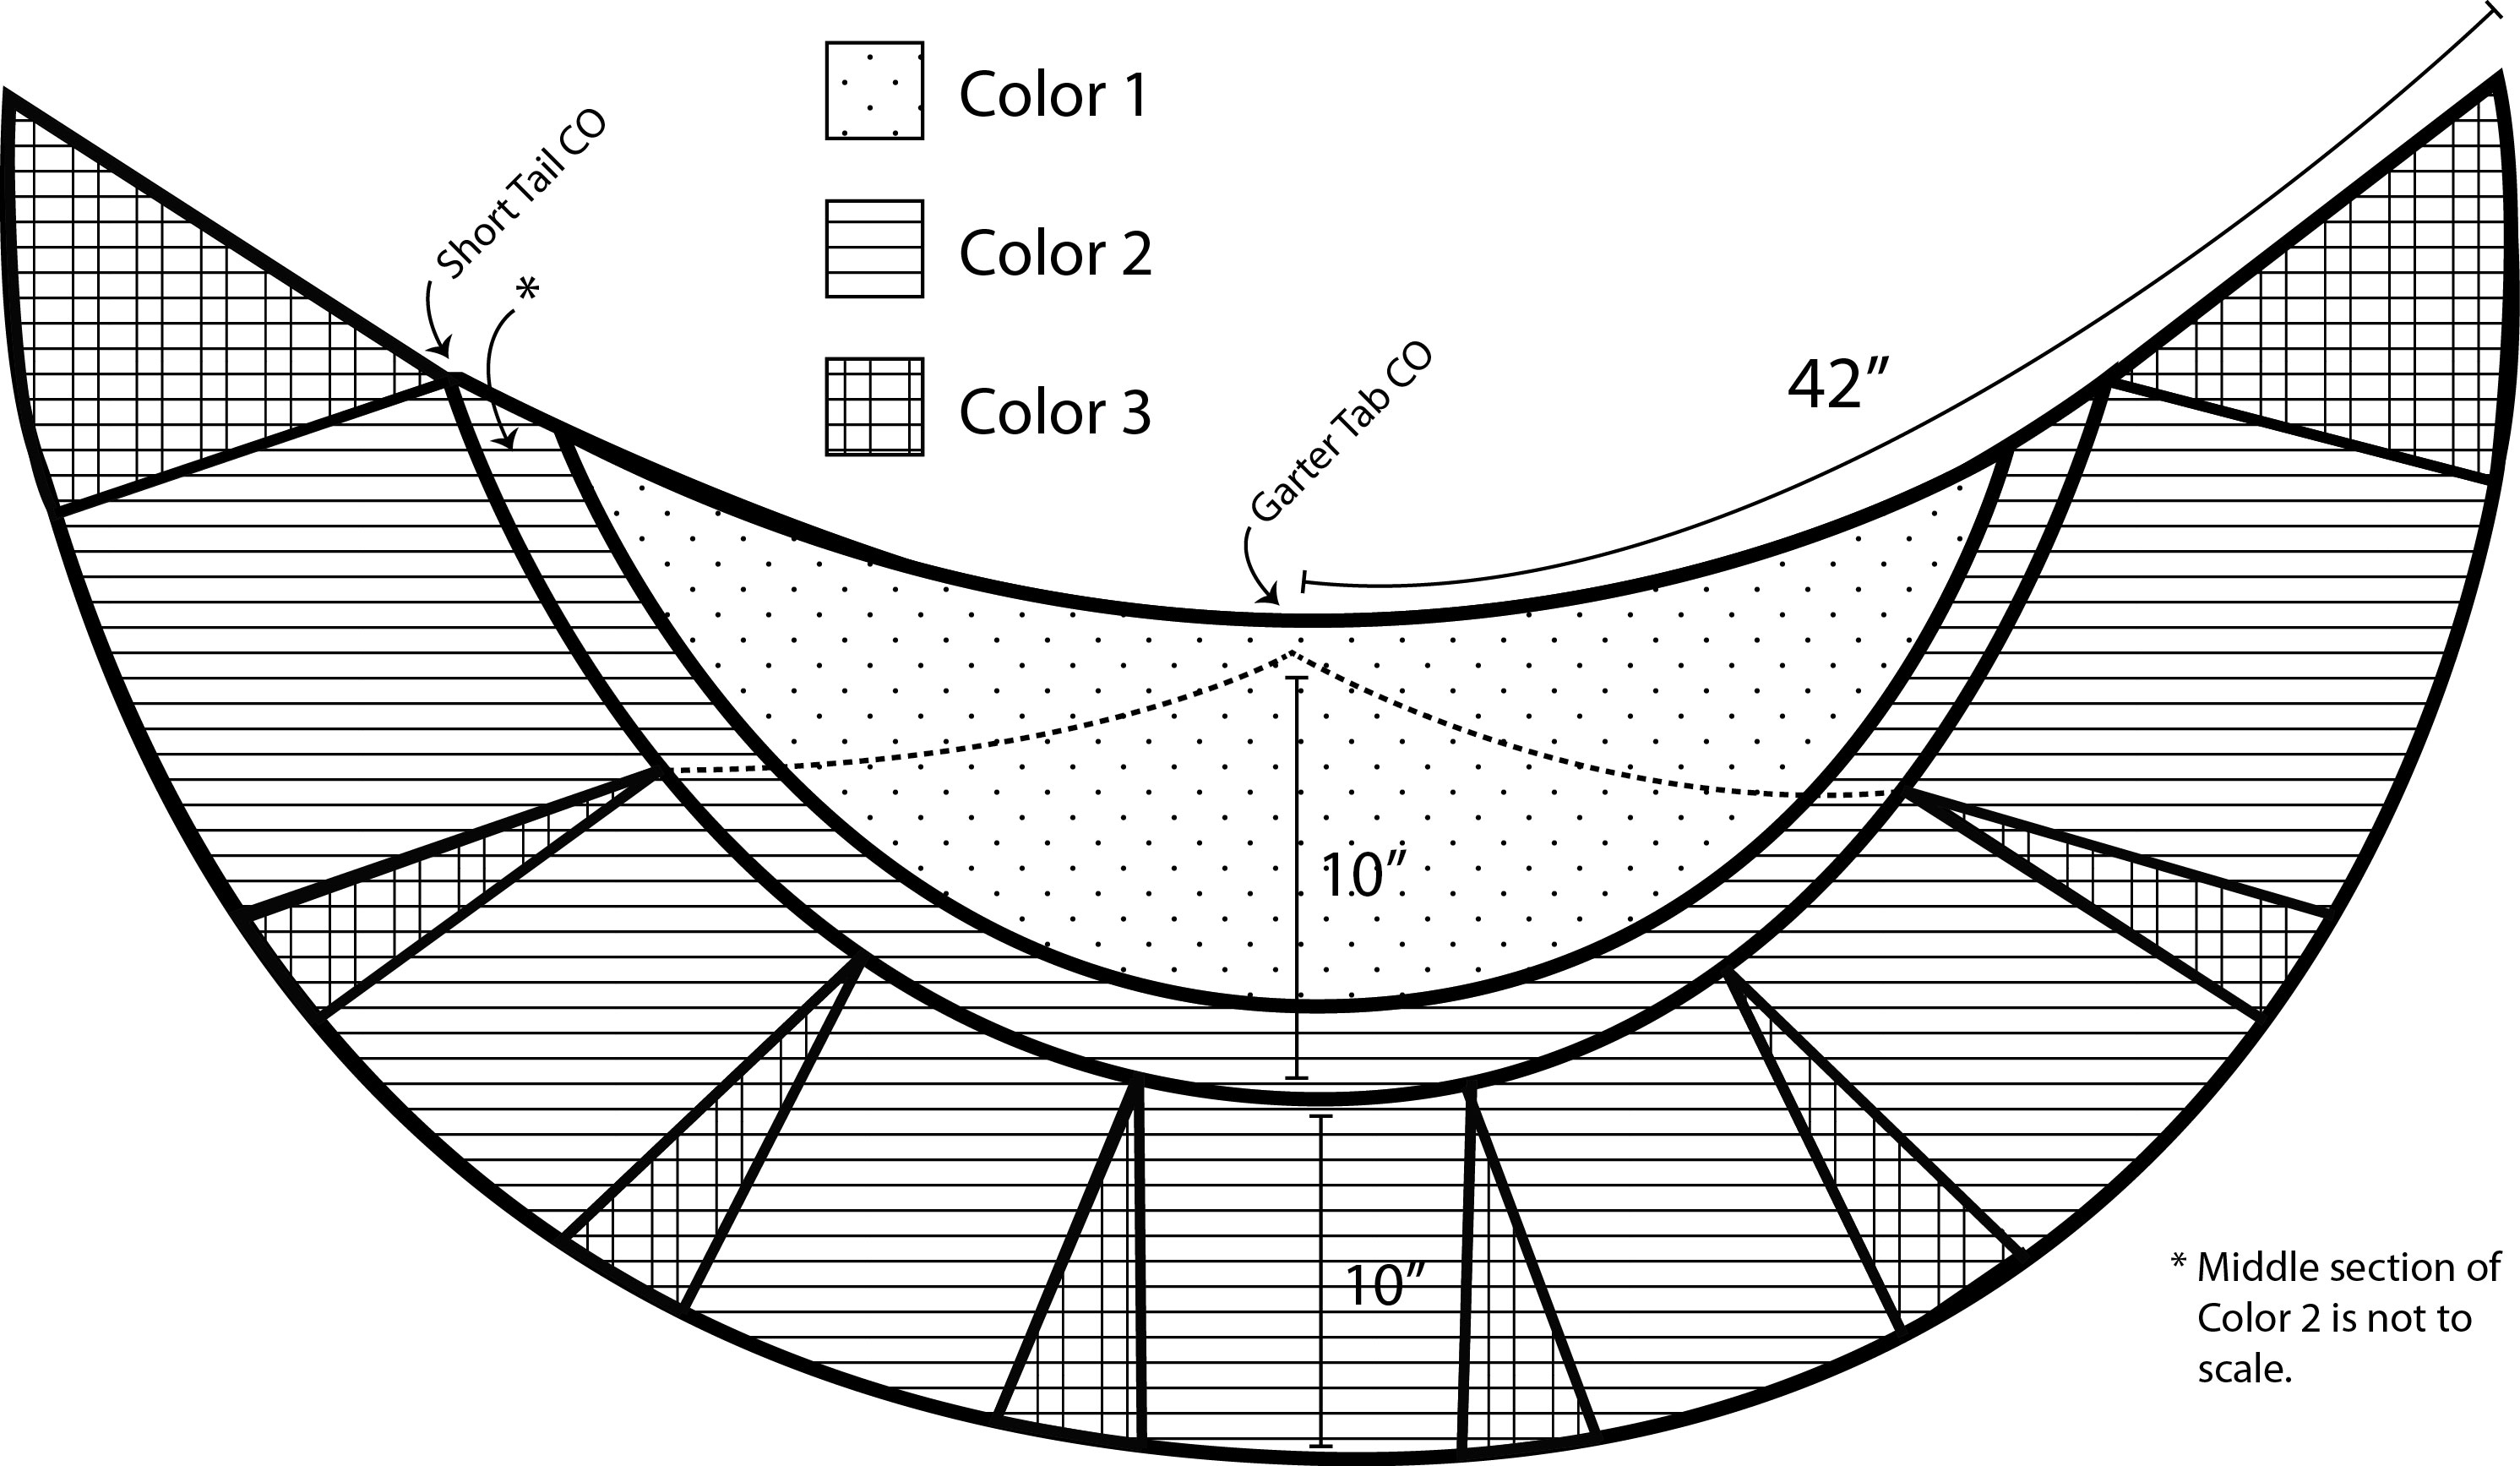
\includegraphics[height=3.5in]{schematic4}
\end{center}

\vfill

\subsection*{Pattern Key}

\vocab{Written instructions:} 

Repeats are indicated with either \textbf{[stitches]} x number \emph{or} \textbf{[stitches]} to specified point.
\vspace{-1em}
\small
\begin{center}
{\renewcommand{\arraystretch}{1.5}
\begin{tabular}{| C{0.1\linewidth}  p{0.9\linewidth} | }
\thickhline \rowcolor{shadecolor} 
\textbf{Abbr.}	& \textbf{Description} \\ \thickhline
 k	&  knit \\
 p	& purl   \\ 
s1	& \textbf{slip one:} slip one st purlwise; wyib -- \mbox{``with yarn in back" \emph{or} \linebreak wyif -- ``with yarn in front"} \\
kfb	& \textbf{knit front back:} knit stitch through front loop as usual, then in the same stitch, knit through the back loop \\
kyok	& \textbf{knit yarn-over knit:} in a single stitch, knit, yarn over, then knit again \\
k2tog 	& knit 2 together \\
p2tog 	& purl 2 together \\
psso & pass slipped st over \\
w\&t & \textbf{wrap \& turn:} s1 wyib, bring yarn to front, s1 back to left needle to ``wrap" stitch, turn work \\
br st	& \textbf{brush stitch:} K1. Insert right needle into third st below the first st on left needle and draw through a loop, leaving it on the needle. K1. Insert needle into same st as before and draw through another loop. K1. Insert needle into same st and draw through a third loop. \mbox{\emph{(See photo tutorial in Appendix.)}} \\
\hline
\end{tabular}
}
\end{center}

\normalsize
\newpage

\begin{multicols}{2}
\begin{frnote}
\textbf{TIP:} When breaking yarns, leave a long (6 in) tail for weaving in.
\end{frnote}

\section*{Cast On and Set Up}

\begin{enumerate}
\item \textbf{Garter tab:} With Color 1, CO 3 sts \mbox{using} the long-tail method. Knit 6 rows in garter stitch. \stitchcount{3} 
\item \vspace{-.5em} After the last row, do not turn work and instead, rotate work by 90 degrees clockwise. Pick up and knit 3 stitches into the garter edge. \stitchcount{6}
\item \vspace{-.5em }Rotate work 90 degrees clockwise again. Pick up and knit 3 stitches along the cast on edge. \stitchcount{9}
\end{enumerate}

Continue with Color 1 and work the following rows once.

\begin{unframed}
\rowDir{Set Up} (WS) k3, yo, k3, yo, k3 \stitchcount{11} \\
\rowDir{Row 1} (RS) k3, kyok into yo, k to 4 sts \\ before end, kyok into yo, k3 \stitchcount{15} \\
\rowDir{Row 2} (WS) k3, yo, k to 3 sts before end, yo, k3 \stitchcount{17} \\
\rowDir{Rows 3-4} Repeat Rows 1-2 \stitchcount{23} \\
\rowDir{Rows 5-6} Repeat Rows 1-2 \stitchcount{29} \\
\rowDir{Row 7} k3, kyok, k9, \pm{A}, k3, \pm{B}, k9, kyok, k3 \stitchcount{33} \\
\rowDir{Row 8} Repeat Row 2, slipping markers (\sm) as they come \stitchcount{35}
\end{unframed}

Reading from right to left, your stitches should look like: 16 sts / A / 3 sts / B / 16 sts \\ = 35 sts total

\vfill

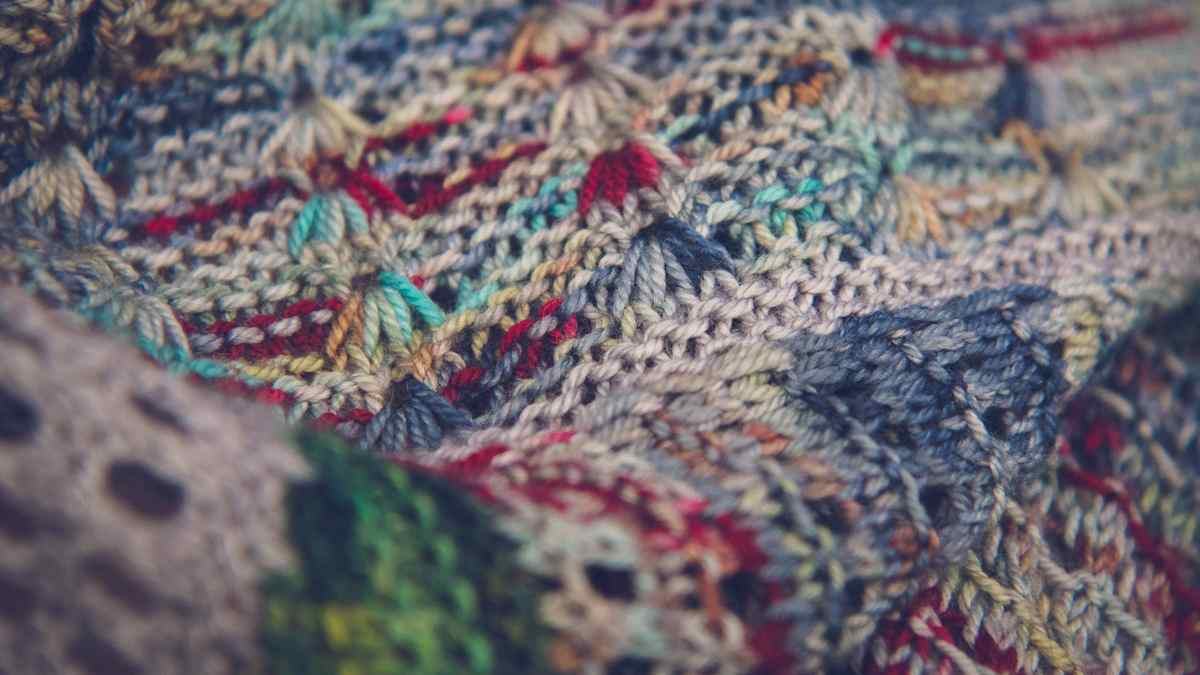
\includegraphics[width=\linewidth]{brushdetail}
\vfill

\columnbreak

\section*{Section 1: Downtown Arts}

Continuing in Color 1, work 12 repeats of Rows 1-6. Total stitch count will increase 18 sts per repeat. In the first repeat, Row 6 should have 3 br sts. In the last (12th) repeat, Row 6 should have 25 br sts. 

\begin{unframed}
\rowDir{Row 1} (RS) k3, kyok into yo, k to 4 sts \\ before end, kyok into yo, k3 \\
\rowDir{Row 2} (WS) k3, yo, k to 3 sts before end, yo, k3 \\
\rowDir{Rows 3-4} Repeat Rows 1-2. \\
\rowDir{Row 5} k3, kyok, k to 6 sts before marker A, \pm{for new A}, br st, k3, \rm{A}, \repeat{br st, k3} to 3 sts from marker B, br st, \rm{B}, k3, br st, \pm{for new B}, k to 4 sts before end, kyok, k3 \\
\rowDir{Row 6} k3, yo, k to marker B, \sm{}, \repeat{p2tog\x3, k3} to 6 sts before marker A, p2tog\x3, \sm{}, k to 3 sts before end, yo, k3
\end{unframed}

% leave long tail

Break Color 1. You should have 52 sts / A / 147 sts / B / 52 sts = 251 sts total 

\section*{Section 2: Steel and Green}

In Section 2, you are working a deep knitted-on border, joining to Section 1 as you go. The two main elements of this section are short row wedges in garter stitch and panels in a 4-row mesh railroad stitch.

\subsection*{Set Up}

Join Color 2, the color you will use for the mesh panels. Work the following rows once.
\begin{unframed}
\rowDir{Row 1} k1, kfb, k to 2 sts before marker A, \pm{for new A}, k2, \rm{A}, k28, \pm{C}, \\ \setrepeat{k30, \pm{C}}{3}, k29, \rm{B}, k1, \pm{for new B}, kfb, k to end \\
\rowDir{Rows 2-4} k across, \sm {} as they come
\end{unframed}
Break Color 2. Your shawl should now be \\ separated into 7 sections: 51 sts / A / 30 sts / C / 30 sts / C / 30 sts / C / 30 sts / C / 30 sts / B / 52 sts  = 253 sts total

\vfill
\newpage

\begin{framed}
\textbf{Sequence:} Work the following sequence. Wedges are worked in Color 3 and mesh panels in Color 2.
\renewcommand\labelitemi{$\square$}
\begin{itemize}[itemsep=-.5em]
\item \textbf{Large Wedge A}
\item \textbf{Mesh Panel} to marker A
\item \textbf{Small Wedge}
\item \textbf{Mesh Panel} to marker C
\item \textbf{Small Wedge}
\item \textbf{Mesh Panel} to marker C
\item \textbf{Small Wedge}
\item \textbf{Mesh Panel} to marker C
\item \textbf{Small Wedge}
\item \textbf{Mesh Panel} to marker C
\item \textbf{Small Wedge}
\item \textbf{Mesh Panel} to marker B
\item \textbf{Small Wedge}
\item \textbf{Mesh Panel} until 2 sts remain between marker D and end of row
\item \textbf{Large Wedge B}
\end{itemize}
\end{framed}

\small
% FIX FLOW OF ROW DIRECTIONS

\subsection*{Large Wedge A}

Join Color 3 and using a short tail CO such as the cable CO, loosely CO 41 sts. \stitchcount{294 total} Set up as follows:
\begin{unframed}
\rowDir{Set Up 1} s1 wyib, k3, w\&t \\
\rowDir{Set Up 2} k to end
\end{unframed}
Repeat Rows 1-2 until wrapped st is next to the 1st CO st.
\begin{unframed}
\rowDir{Row 1} s1 wyib, k to wrapped st, work wrapped st by inserting needle knitwise into wrap then k together with st \emph{(All wrapped sts worked likewise)}, w\&t \\
\rowDir{Row 2} k to end
\end{unframed}

Work Rows 3-4 once to finish Large Wedge A.

\begin{unframed}
\rowDir{Row 3} s1 wyib, k to wrapped st, work wrapped st, \pm{D} \emph{(marks where Section 1 is joined)}, s1 wyib, k1, psso, turn \decrease{1} \\
\rowDir{Row 4} s1 wyif, \sm{} \emph{D}, k to end
\end{unframed}

 Break Color 3. 
\vspace{1em}

After Large Wedge A, your work should look like: 40 sts / D / slipped st / \emph{rest of shawl...}


\vfill
\columnbreak
\subsection*{Mesh Panel (Railroad Stitch)}

\begin{frnote}
\textbf{TIP:} The mesh panels will always be 40 sts wide.
\end{frnote}

Join Color 2. Repeat Rows 1-4 of the railroad stitch until there are 3 sts between marker D and the \\ specified point. 
\begin{unframed}
\rowDir{Row 1} s1 wyib, k to D, \sm{} \emph{D}, s1 wyib, k2tog, psso, turn \decrease{2} \\
\rowDir{Row 2} s1 wyif, \sm{} \emph{D}, k to end \\
\rowDir{Row 3} s1 wyib, k3, \repeat{yo, k2tog} to marker D, \sm{} \emph{D}, s1 wyib, k1, psso, turn \decrease{1} \\
\rowDir{Row 4} s1 wyif, \sm{} \emph{D}, p to 4 sts before end, k4
\end{unframed} 
Work Rows 1-2 once more and \rm{}when you come to it. Break Color 2.

\subsection*{Small Wedge}

Join Color 3 and repeat Set Up 1-2 from Large Wedge A. Repeat Rows 1-2 until there is 1 st \\ between wrapped st and marker D. \emph{(note the k1 after the wrapped st!)}
\begin{unframed}
\rowDir{Row 1} s1 wyib, k to wrapped st, work wrapped st, k1, w\&t \\
\rowDir{Row 2} k to end \end{unframed}
Work Rows 3-4 once to finish the small wedge. 
\begin{unframed}
\rowDir{Row 3} s1 wyib, k to wrapped st, work wrapped st, k1, \sm{} \emph{D}, s1 wyib, k1, psso, turn \decrease{1} \\
\rowDir{Row 4} s1 wyif, \sm{} \emph{D}, k to end 
\end{unframed}
Break Color 3.

\vspace{1em}
Before beginning Large Wedge B, you will have 42 sts, with two sts between marker D and the end.

\subsection*{Large Wedge B}

Join Color 3. Work Rows 1-2 once.

\begin{unframed}
\rowDir{Row 1} s1 wyib, k to marker D, \rm{D}, s1 wyib, k1, psso, turn \decrease{1} \\
\rowDir{Row 2} s1 wyif, k to end
\end{unframed}

Repeat Rows 3-4 until 3 sts remain.

\begin{unframed}
\rowDir{Row 3} s1 wyib, k to 2 sts before end, k2tog \\ \decrease{1} \\
\rowDir{Row 4} Repeat Row 2
\end{unframed}

Work Rows 5-7 once until 1 st remains.

\begin{unframed}
\rowDir{Row 5} s1 wyib, k2tog \stitchcount{2} \\
\rowDir{Row 6} s1 wyif, k1 \\
\rowDir{Row 7} k2tog \emph{(1 st)}
\end{unframed}

\normalsize
\section*{Finishing}
To finish, break yarn and pull end through the last stitch. Block aggressively. You'll have quite a lot of ends! You can either:
\vspace{-.5em}
\begin{itemize}[itemsep=0mm]
\item weave them all in
\item place a tassel at each color change in Section 2 \emph{(where a wedge and mesh panel meet)} to disguise the ends.
\end{itemize}

\section*{Appendix: Brush Stitch}

Before working the brush stitch, your work should look like this:

\begin{center} 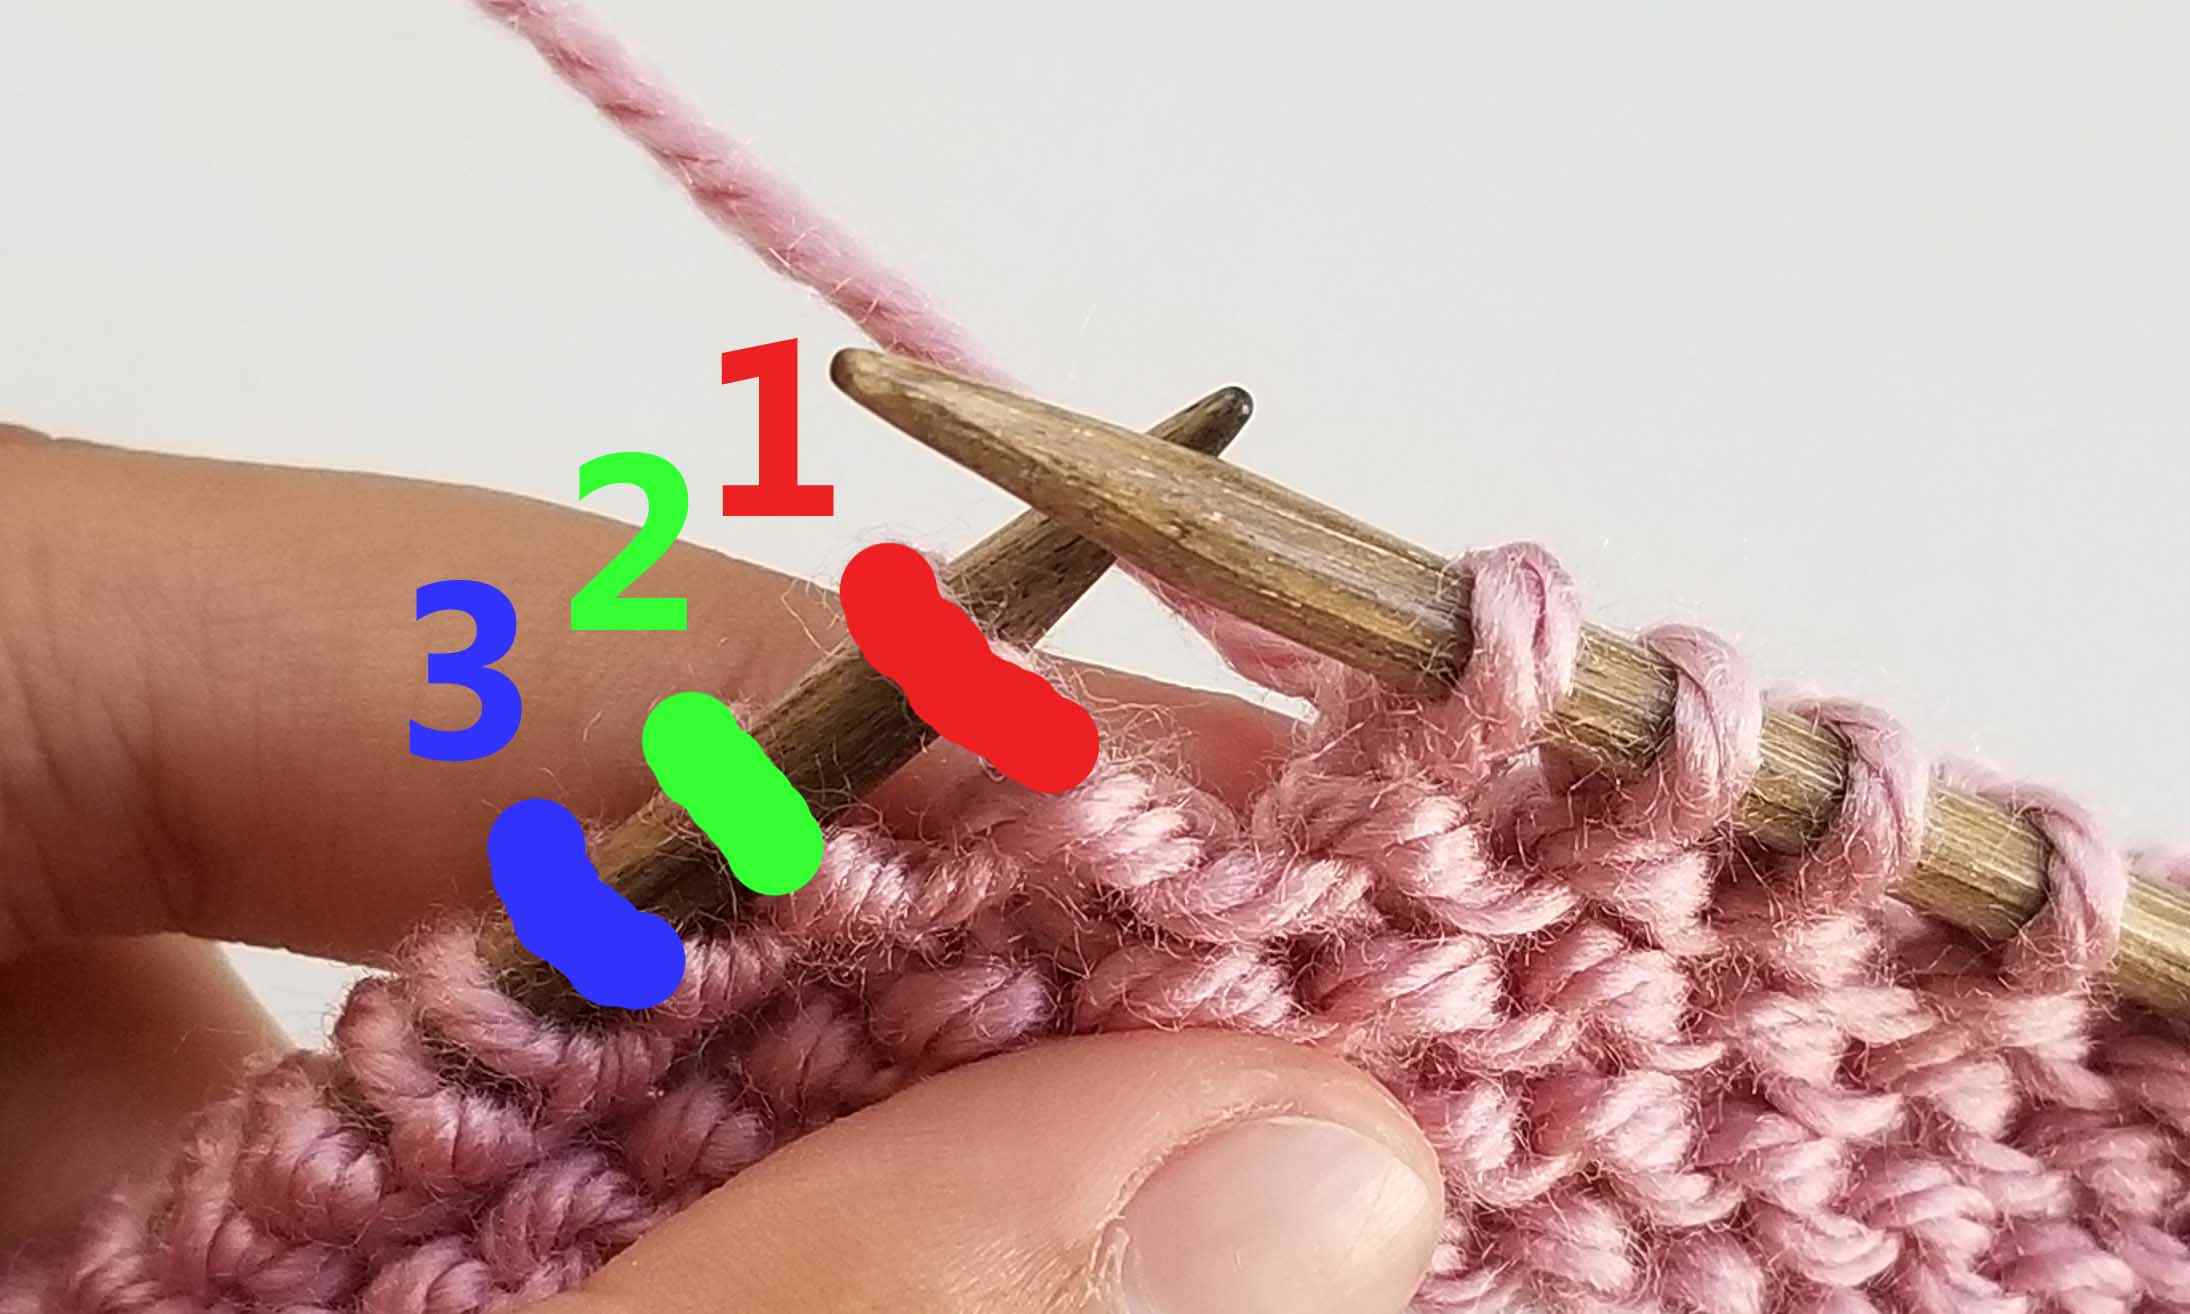
\includegraphics[height=1.5in]{0_setup.jpg}
\end{center}

\begin{enumerate}
\item Knit 1 st. (1) \\ 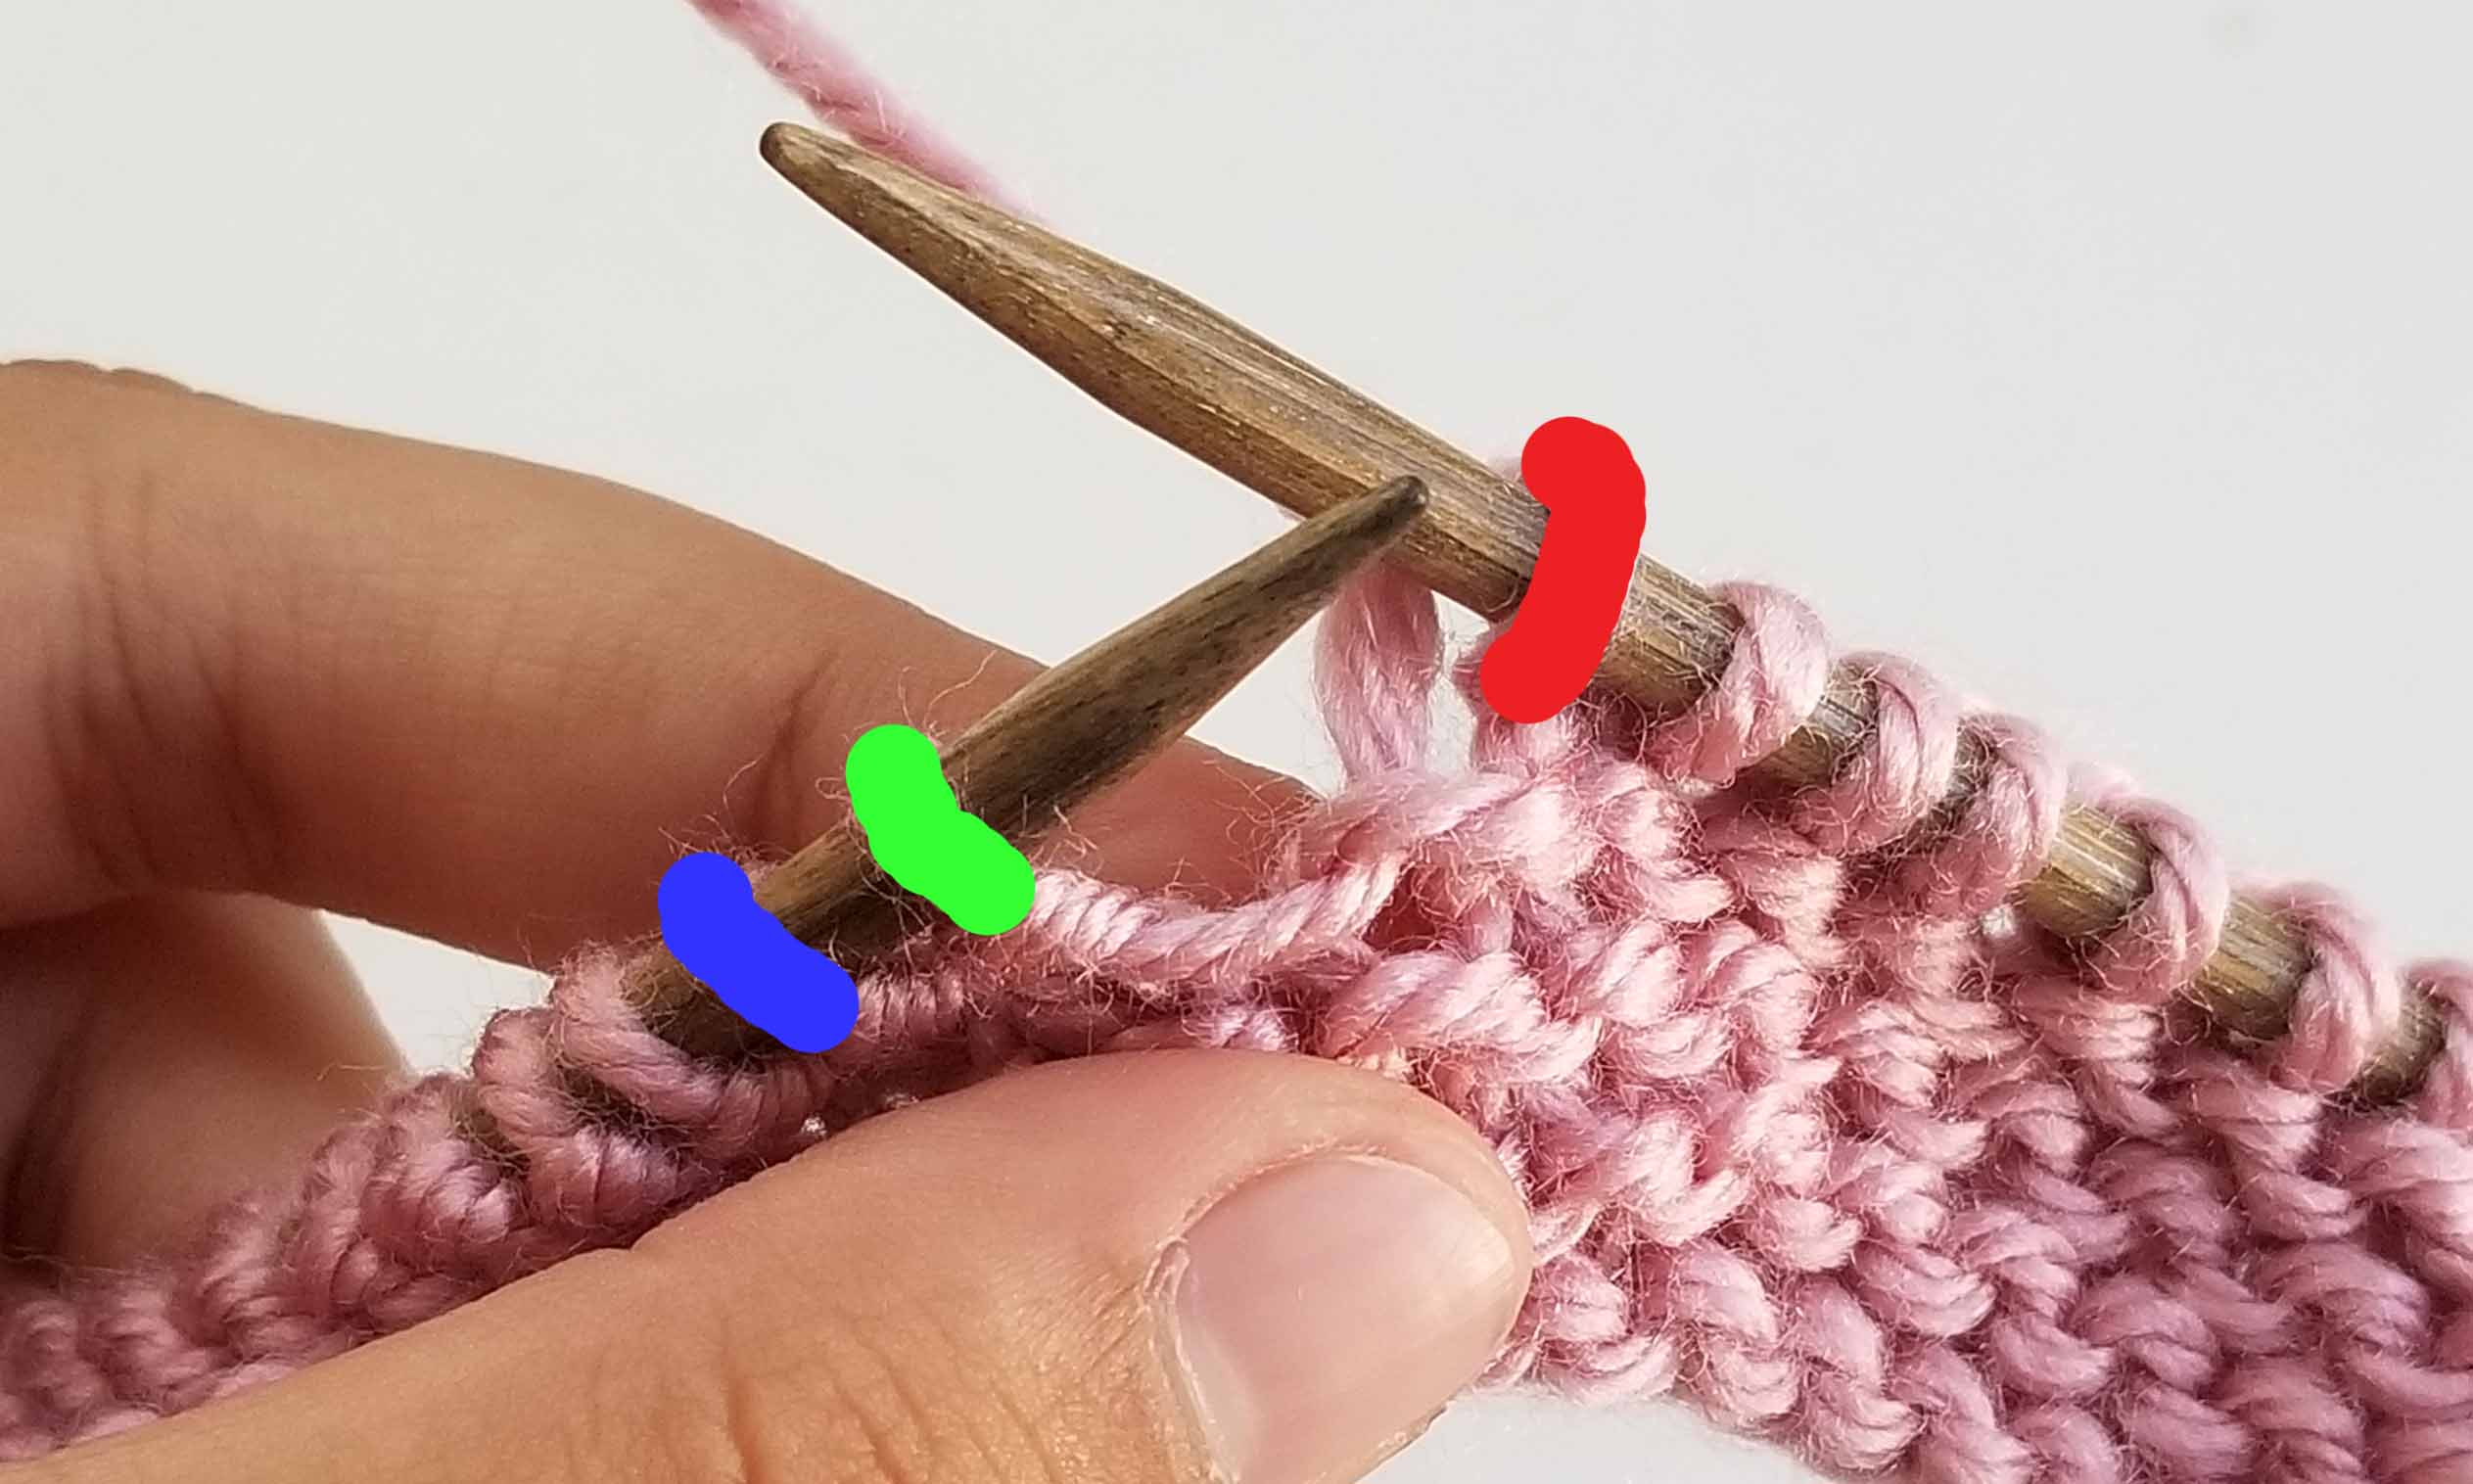
\includegraphics[height=1.5in]{1_knit1.jpg}
\item Insert R needle into third st below the first st (green) on the L needle. \\ 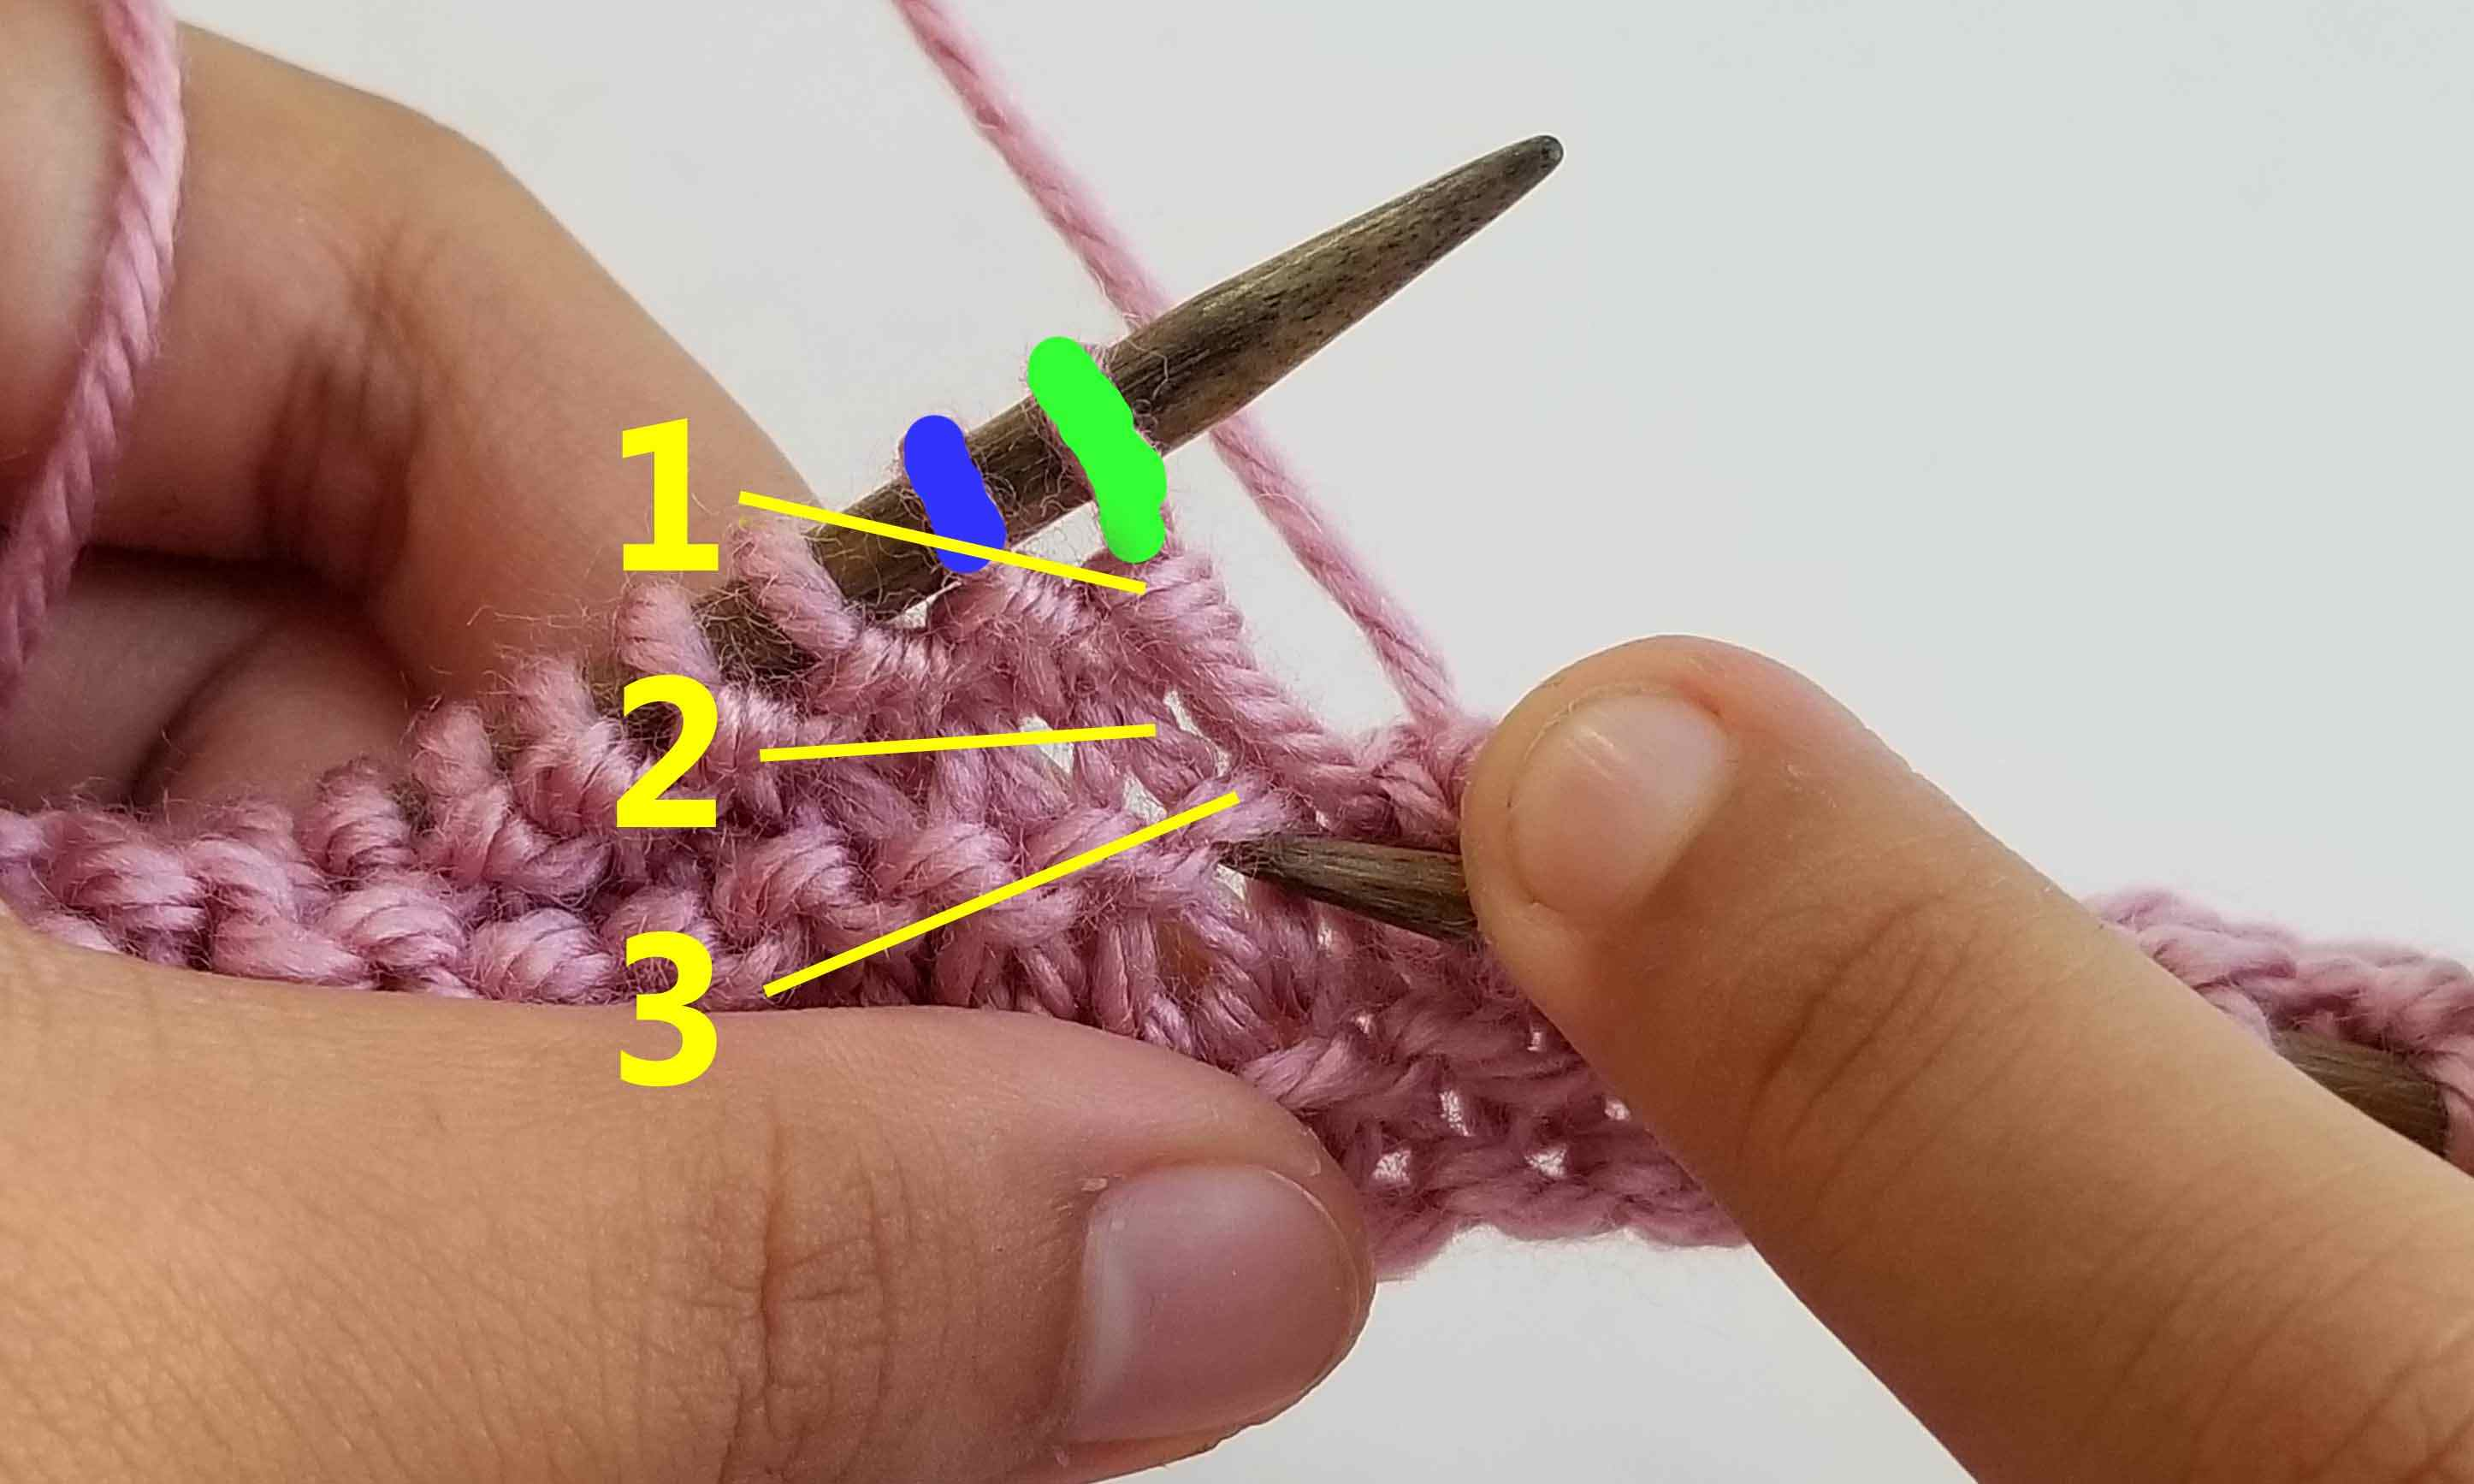
\includegraphics[height=2in]{2_insert.jpg}

\vfill
\columnbreak

\item Draw through a loop, leaving it on the needle. (1a) \\ 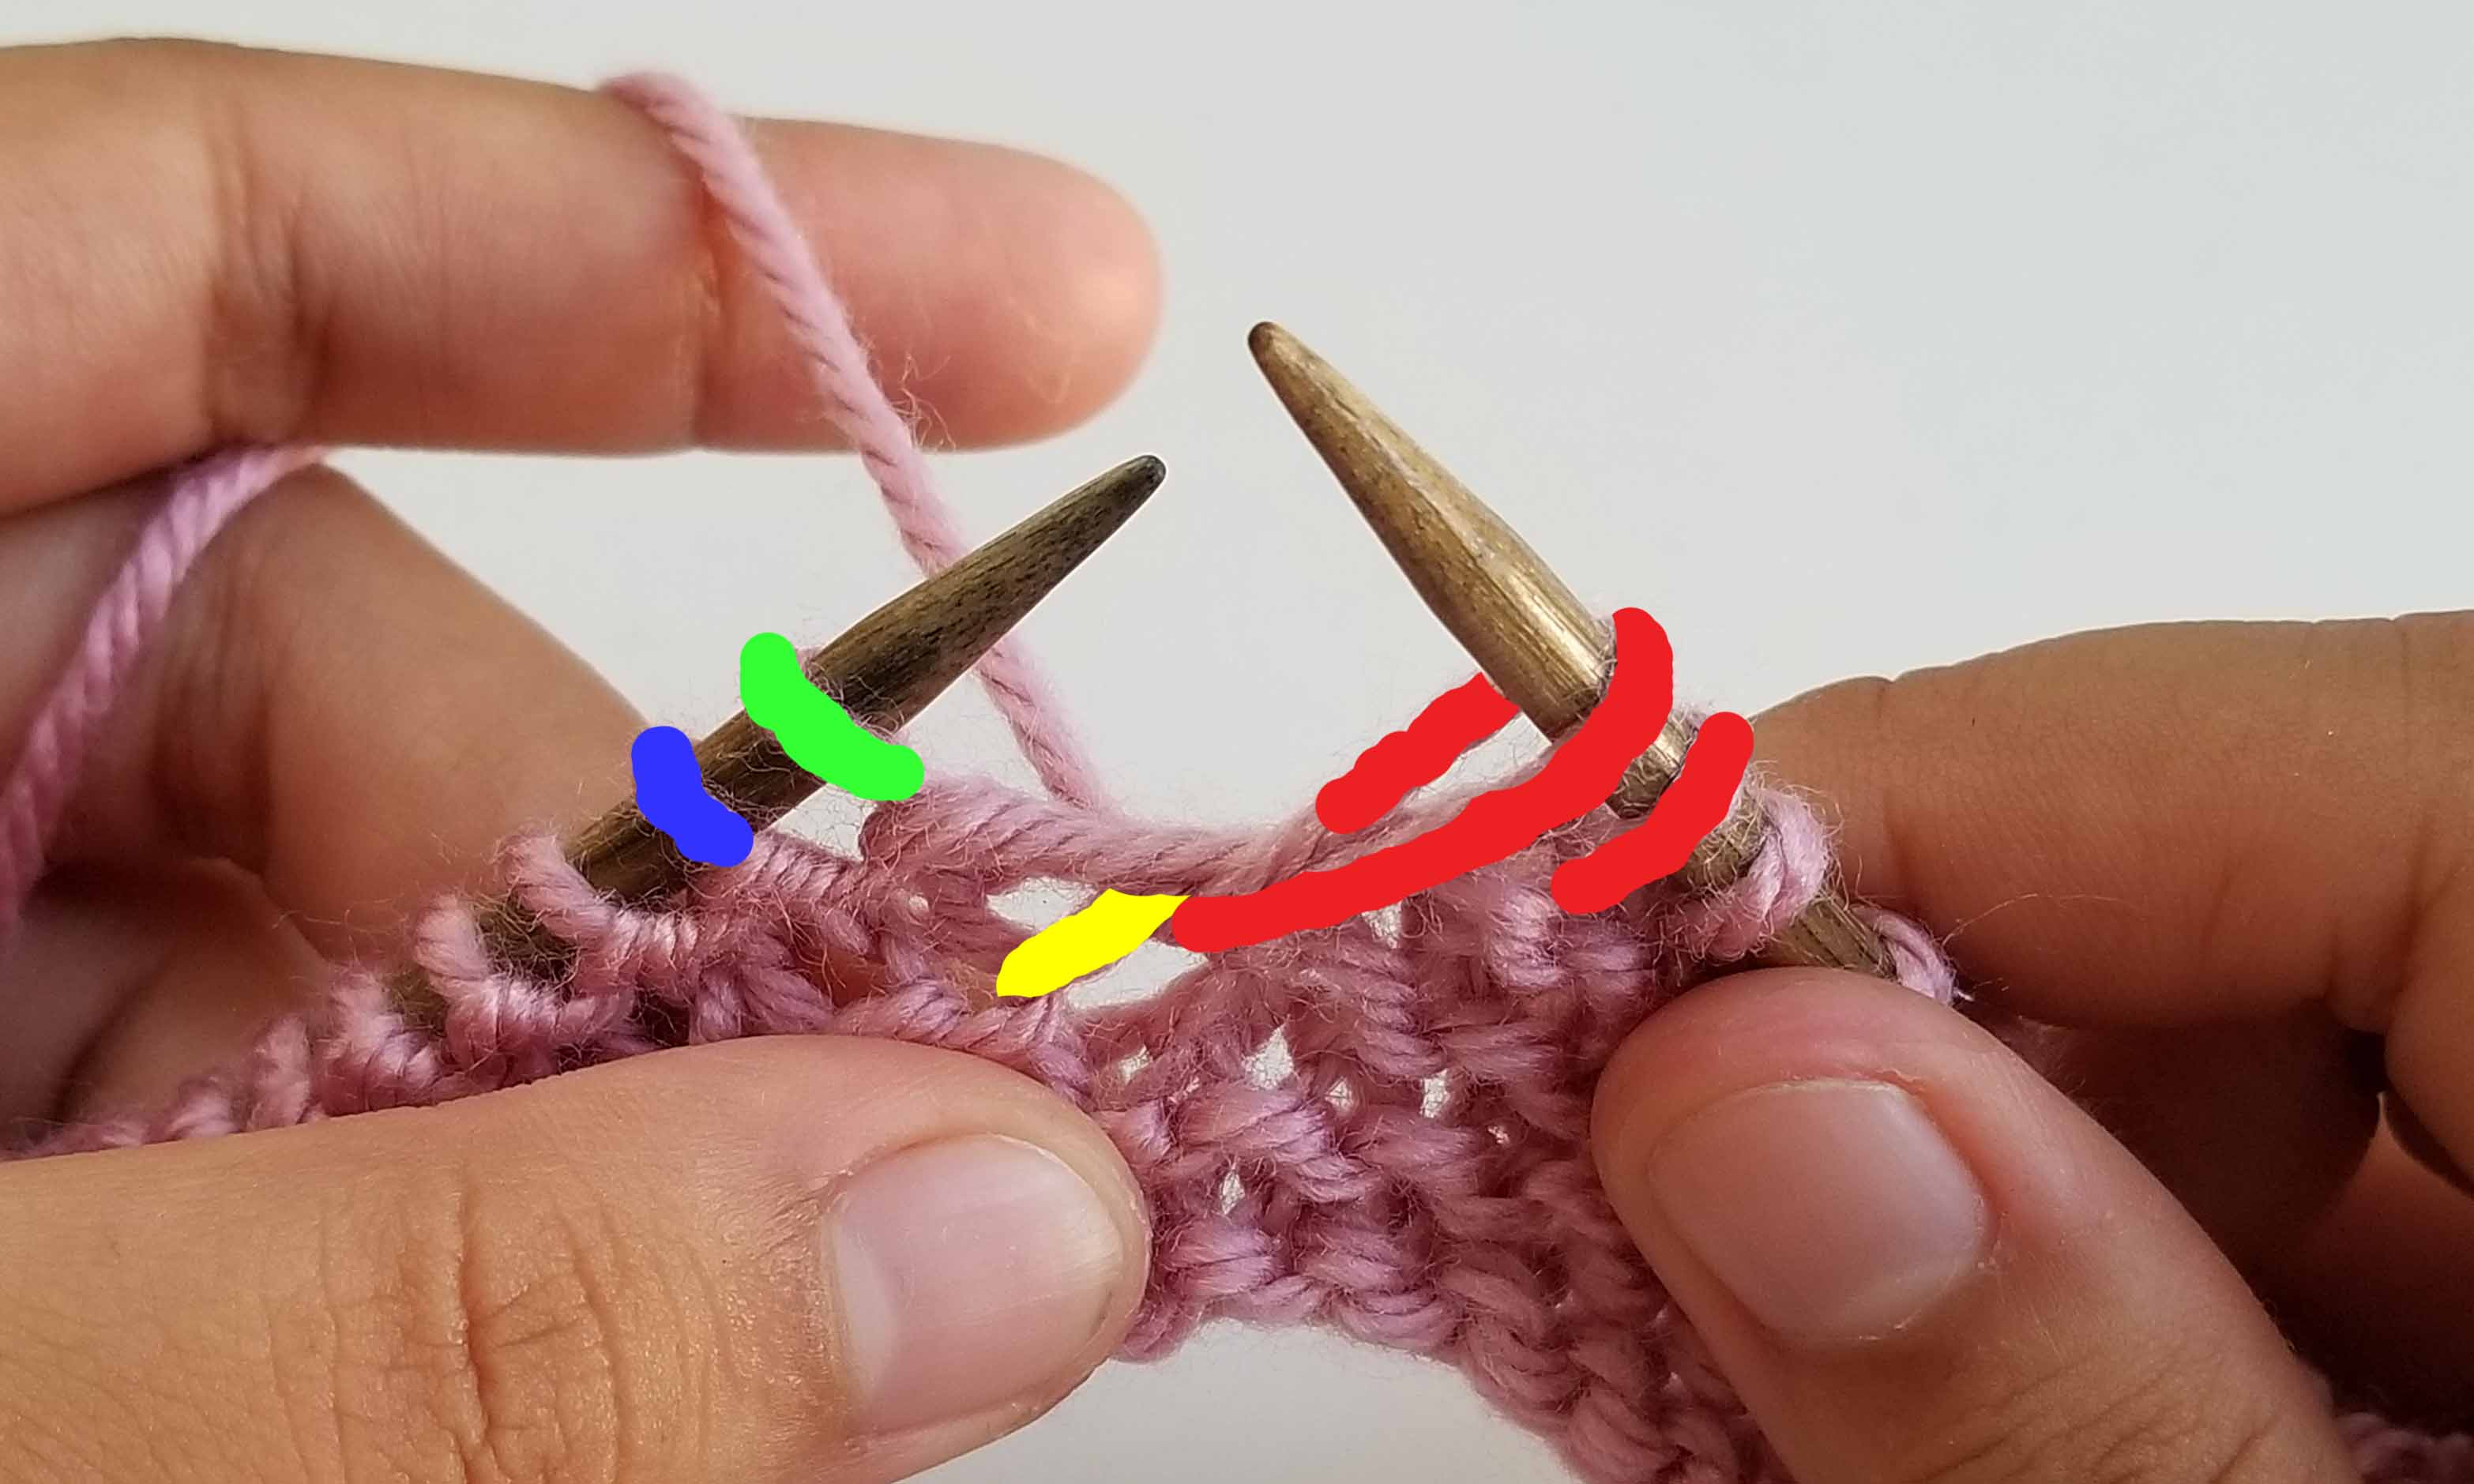
\includegraphics[height=1.5in]{3.jpg}
\item Knit 1 st. (2) \\ 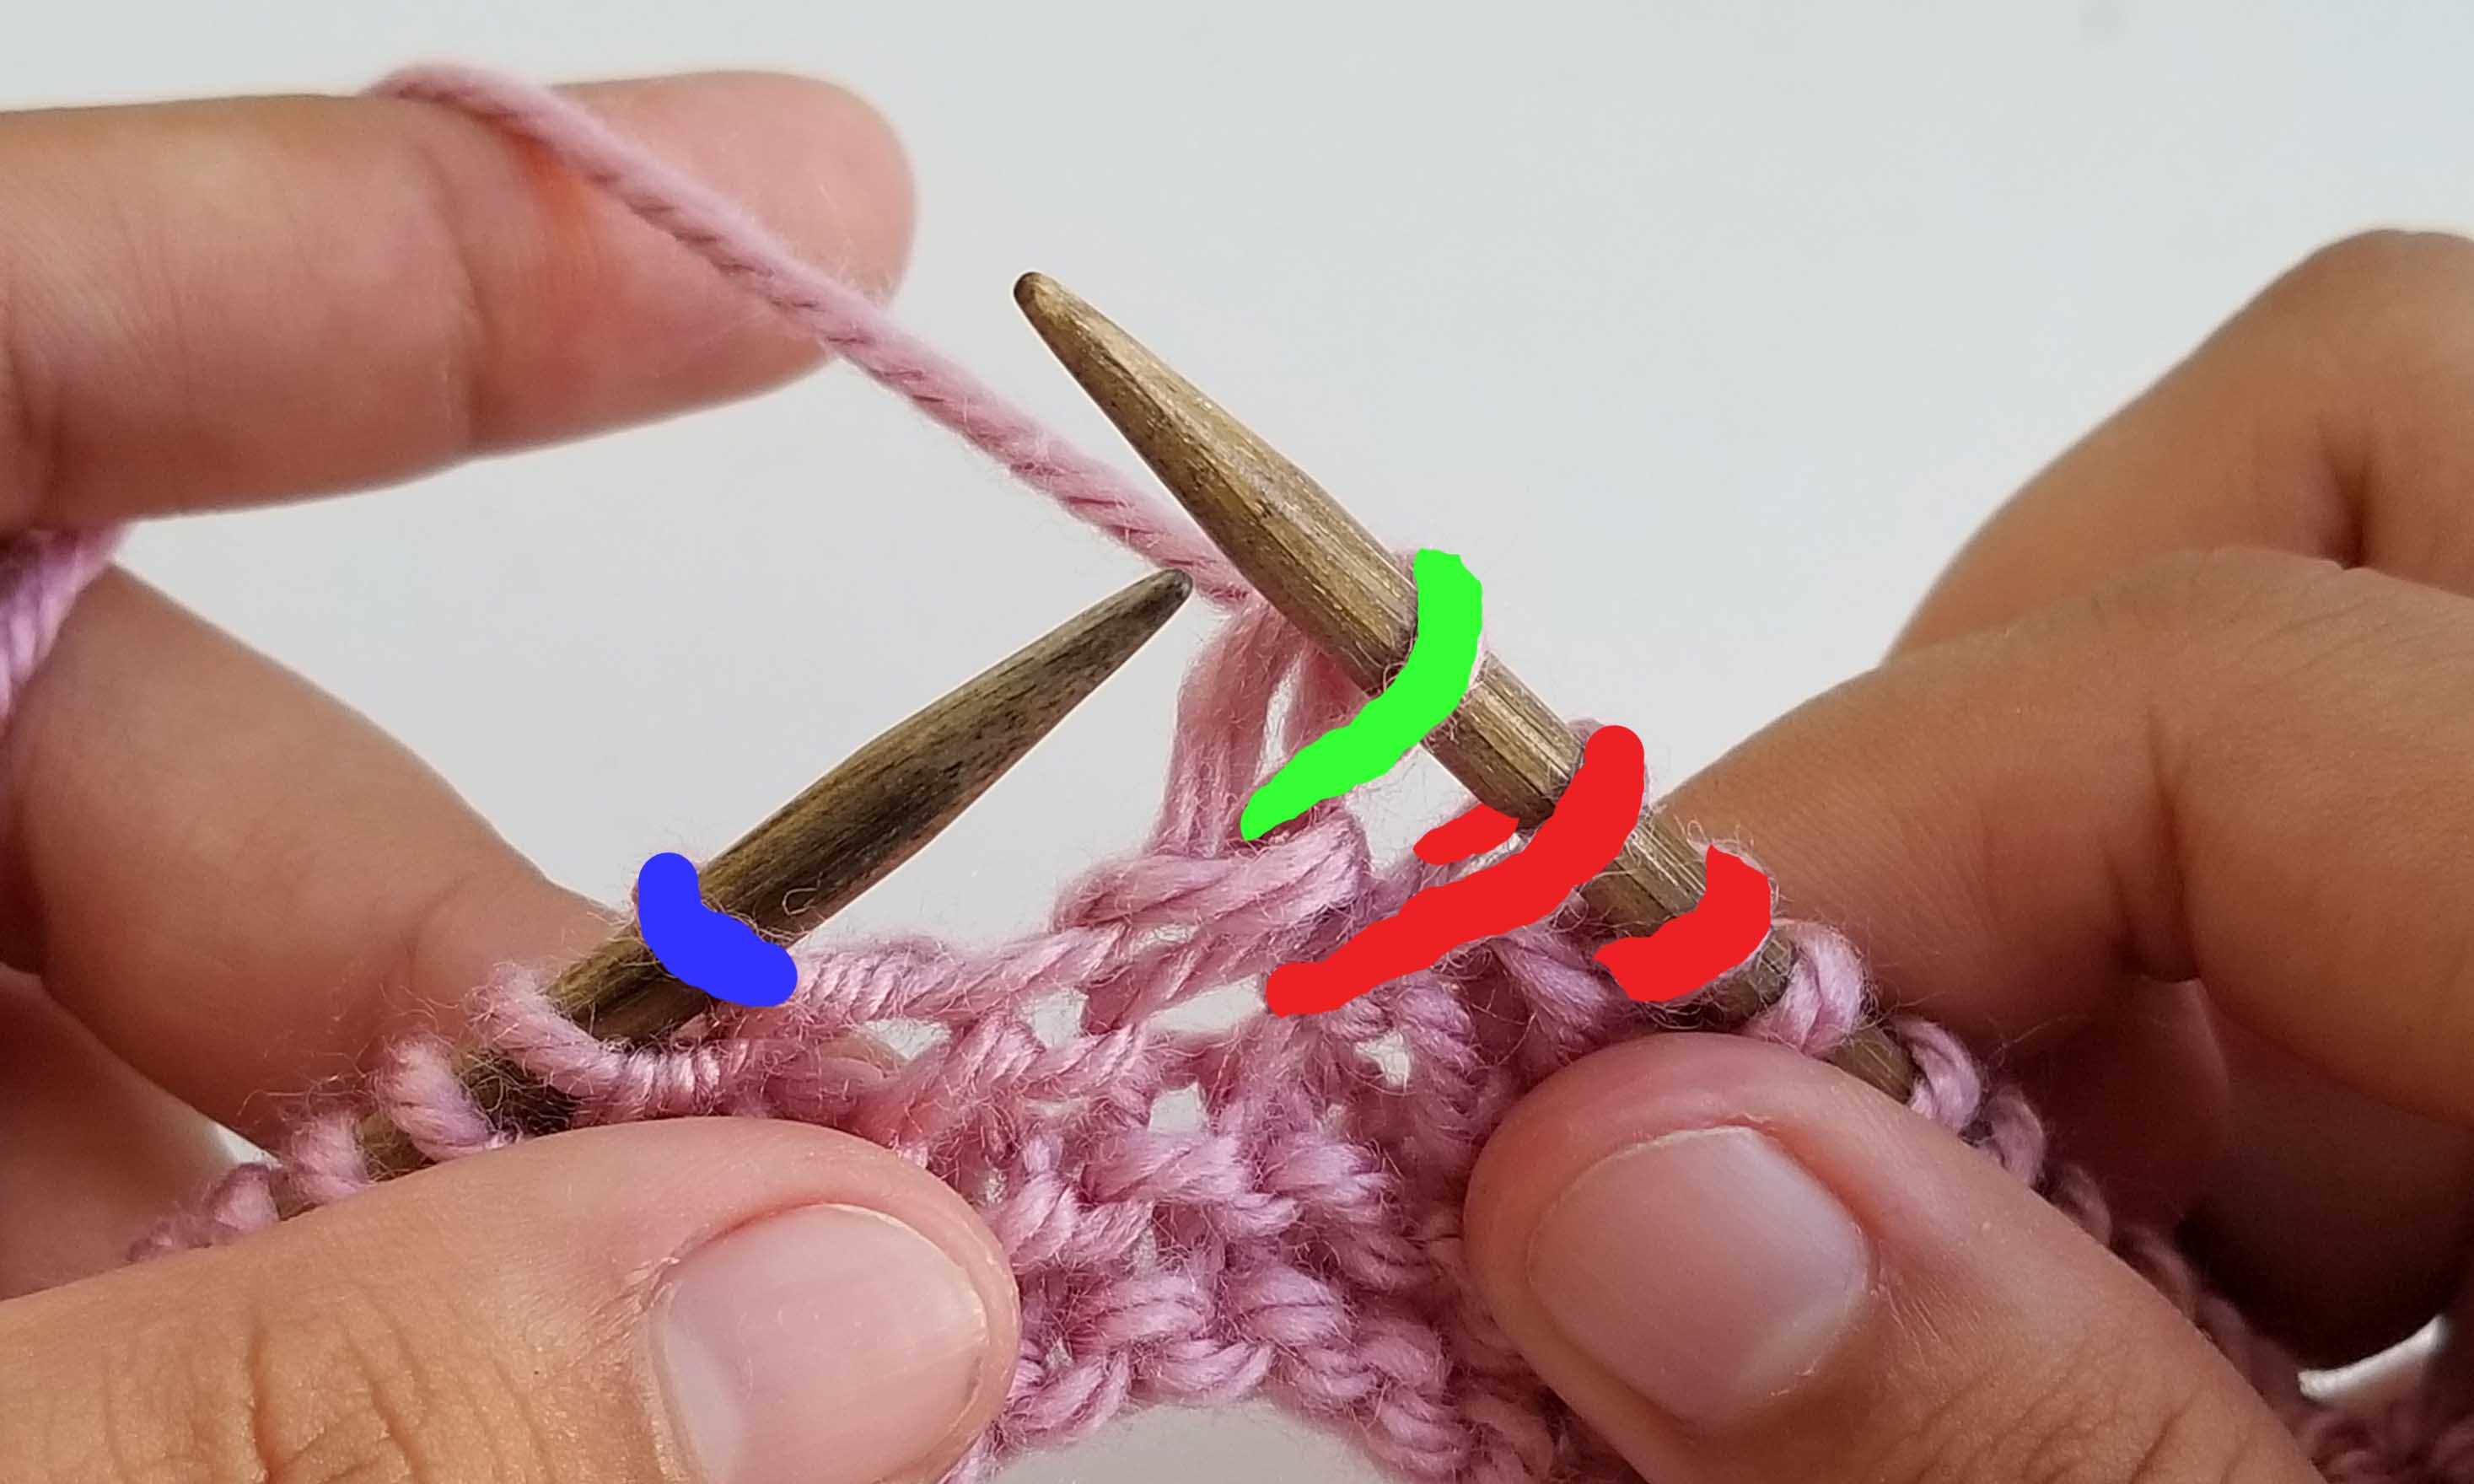
\includegraphics[height=1.5in]{4_knit2.jpg}
\item Insert R needle into same st as before and draw through another loop, leaving it on the needle. (2a) \\ 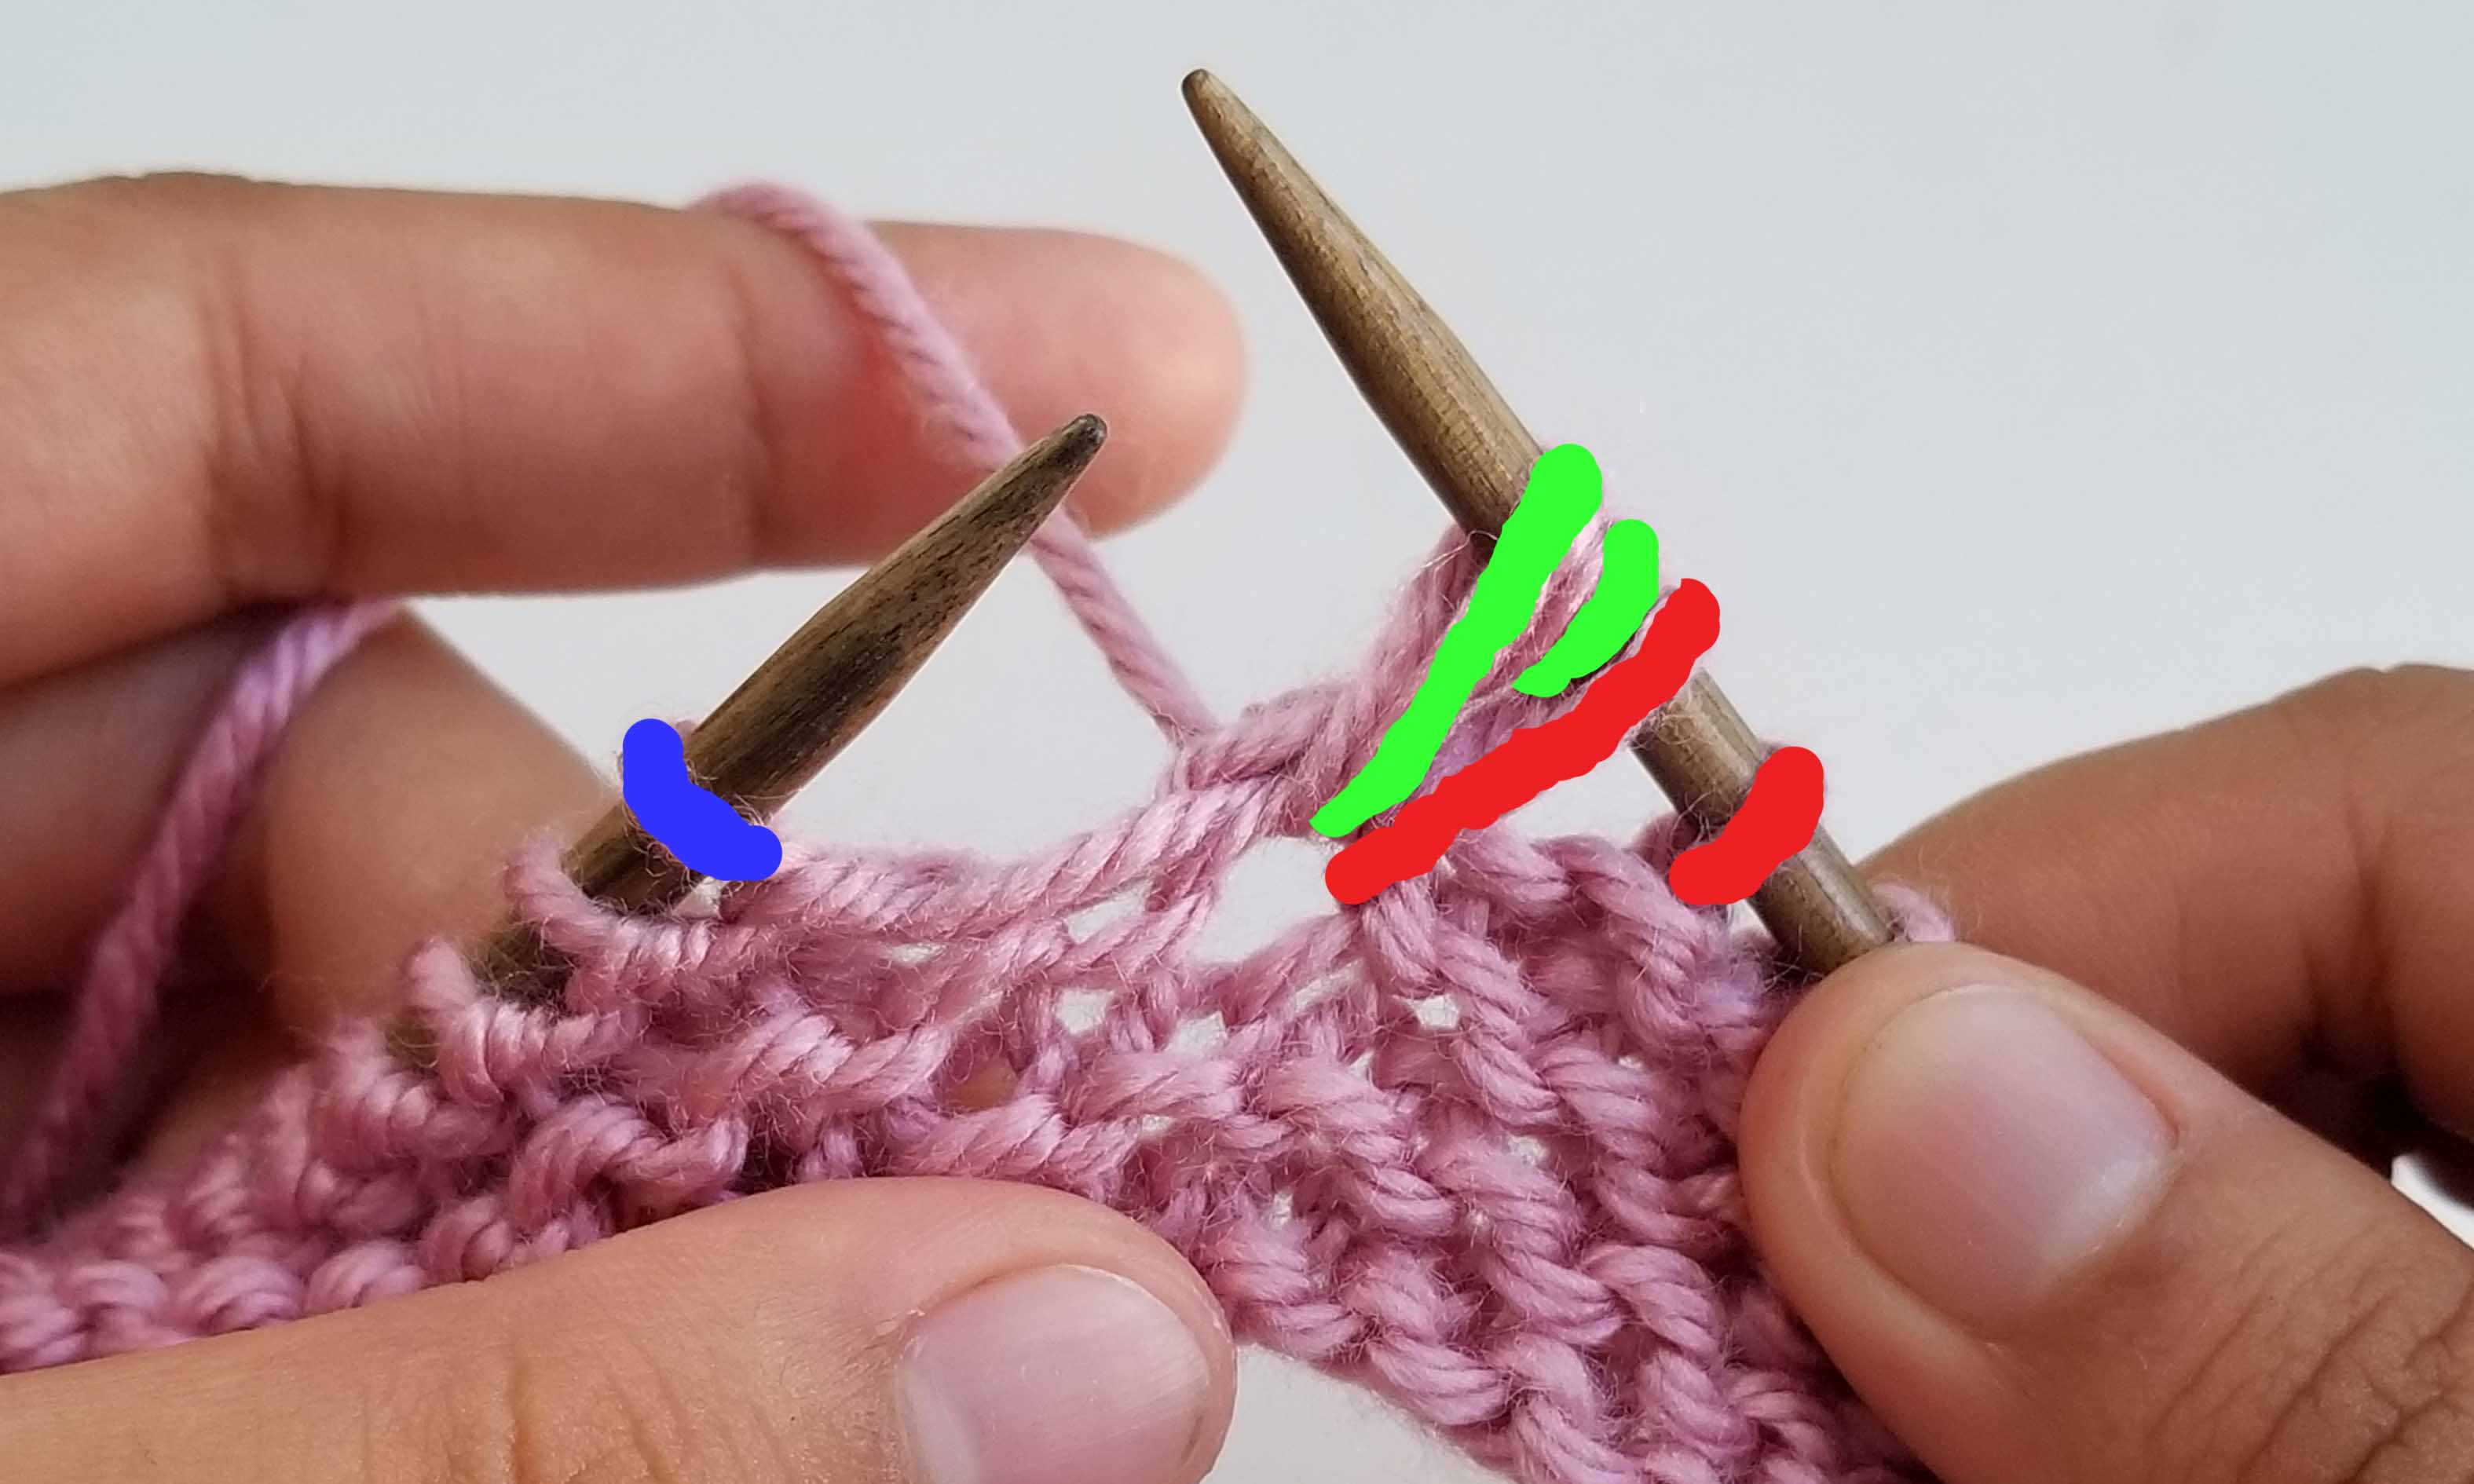
\includegraphics[height=1.5in]{5_loop2.jpg}
\item Knit 1 st. (3) \\ 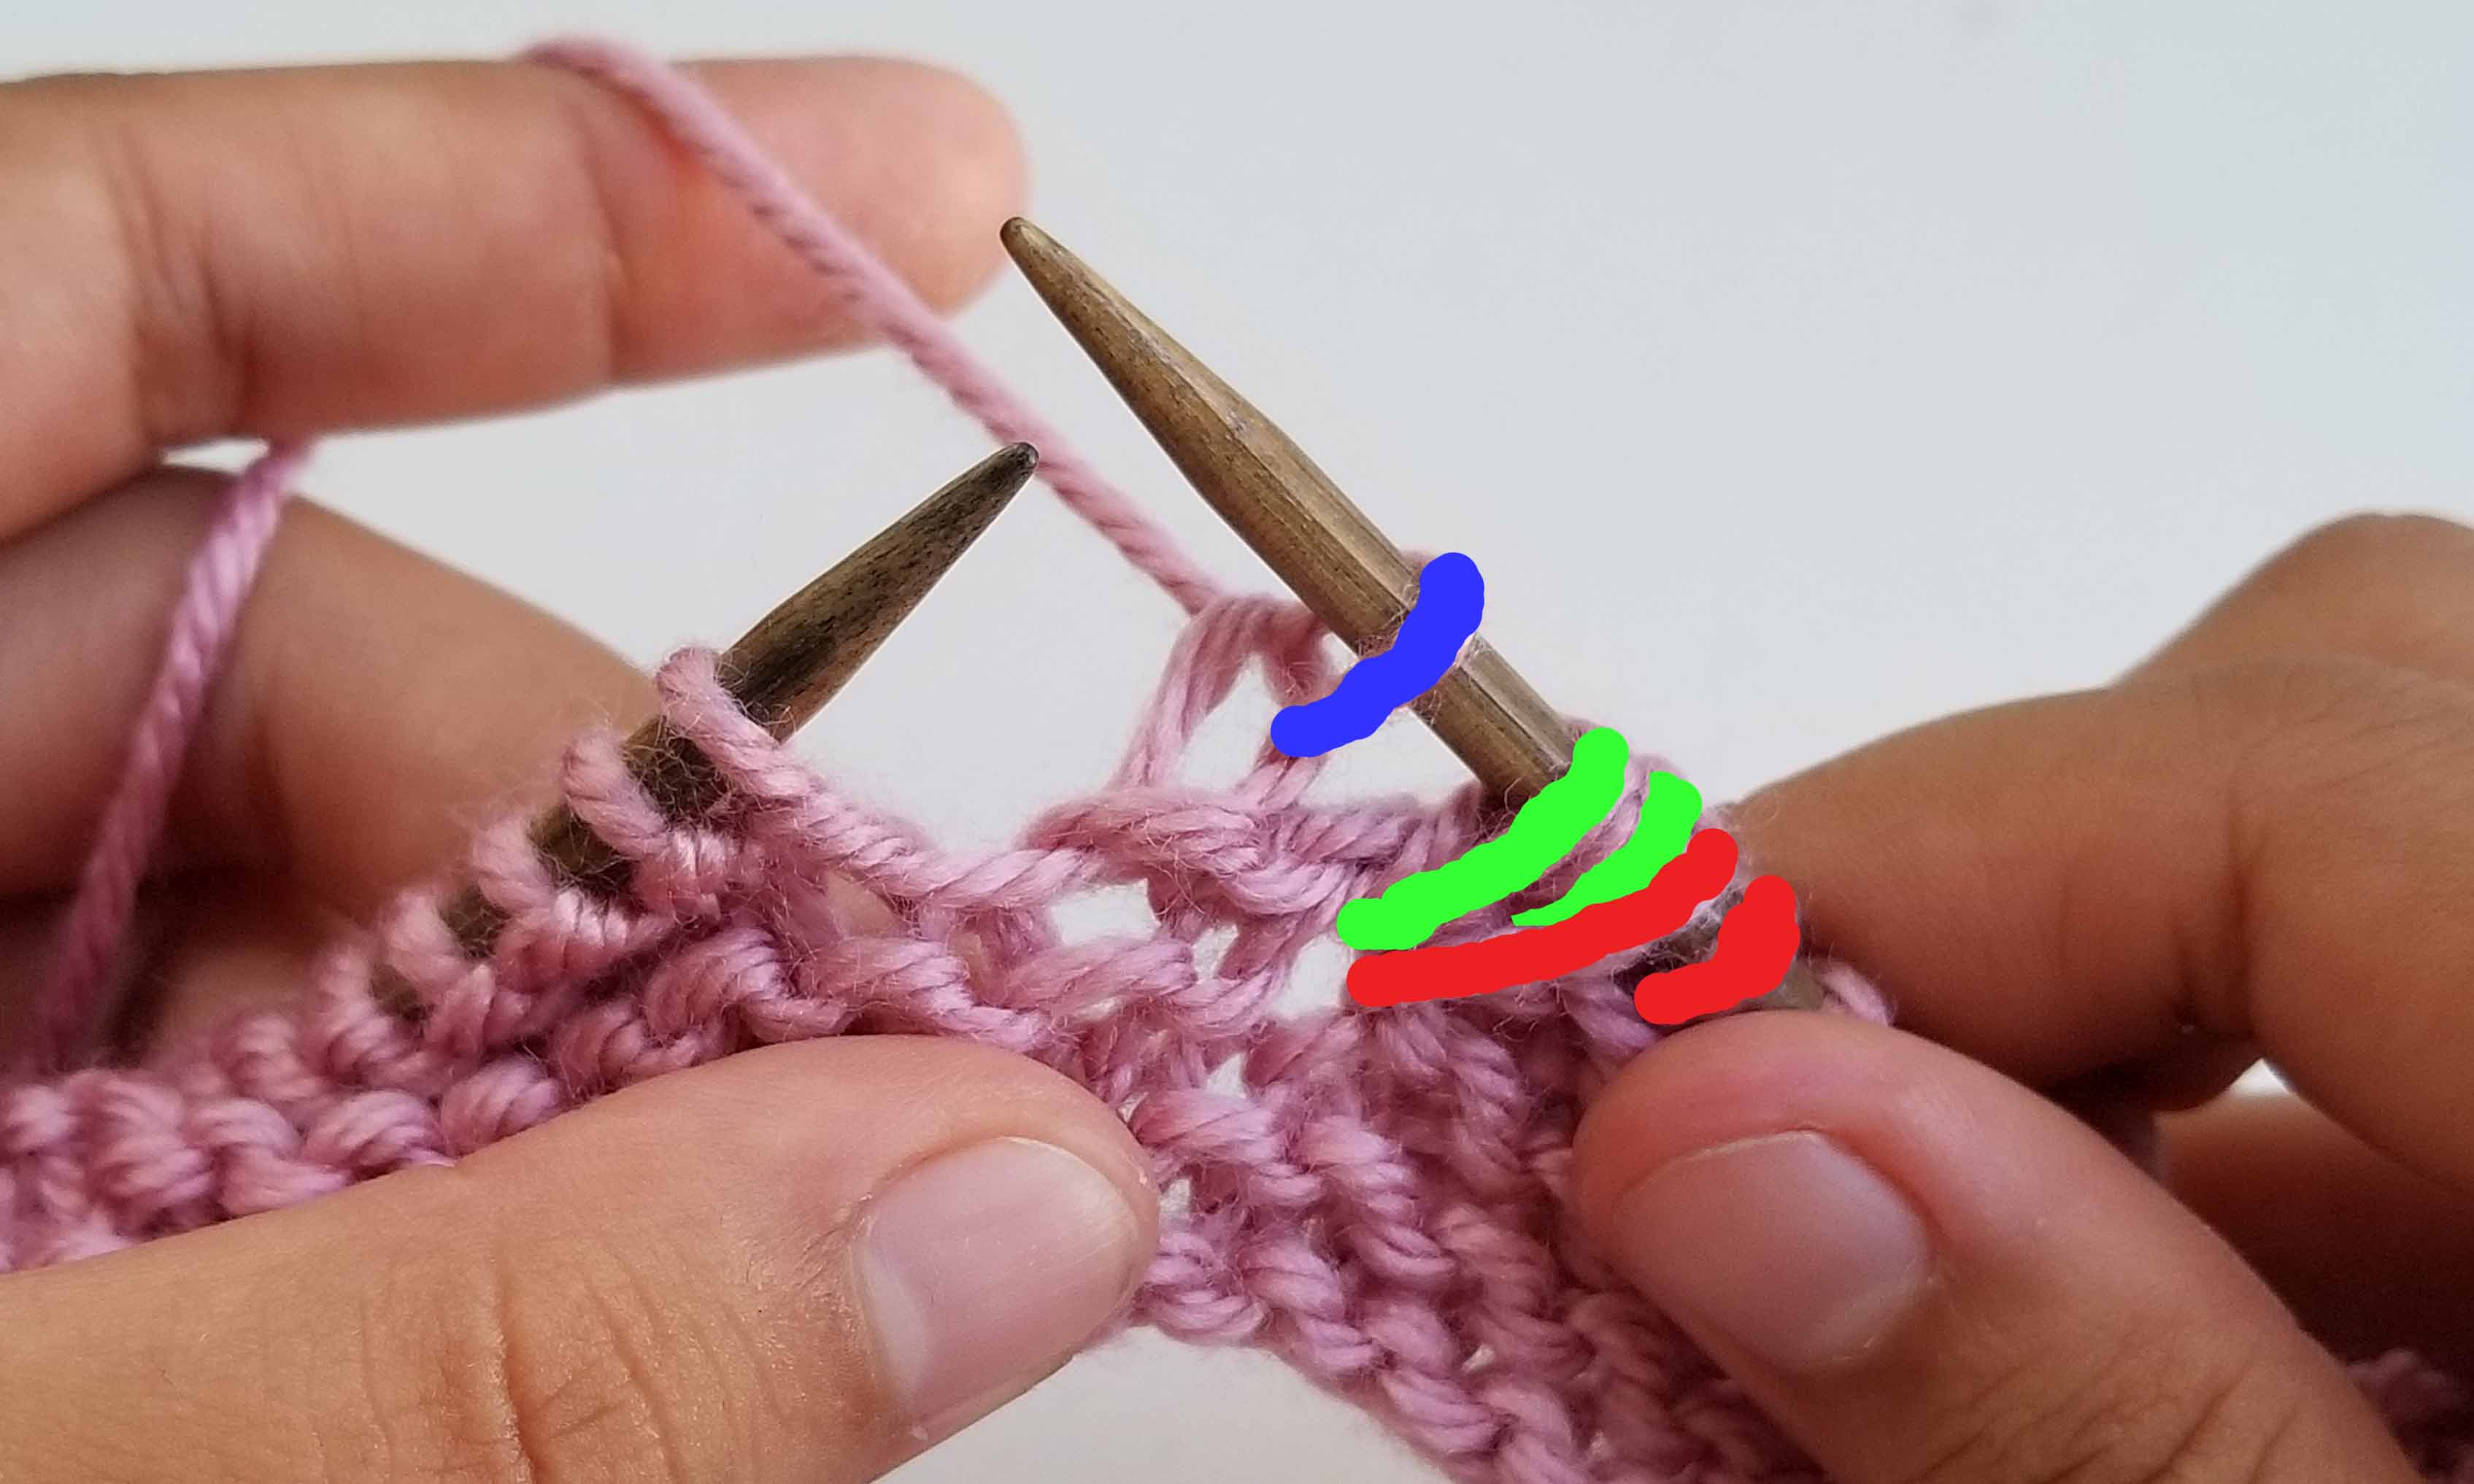
\includegraphics[height=1.5in]{6_knit3.jpg}

\vfill

\newpage

% FIX FLOW OF THIS PAGE

\item Insert R needle into same st and draw through a third loop, leaving it on the needle. (3a) \\ 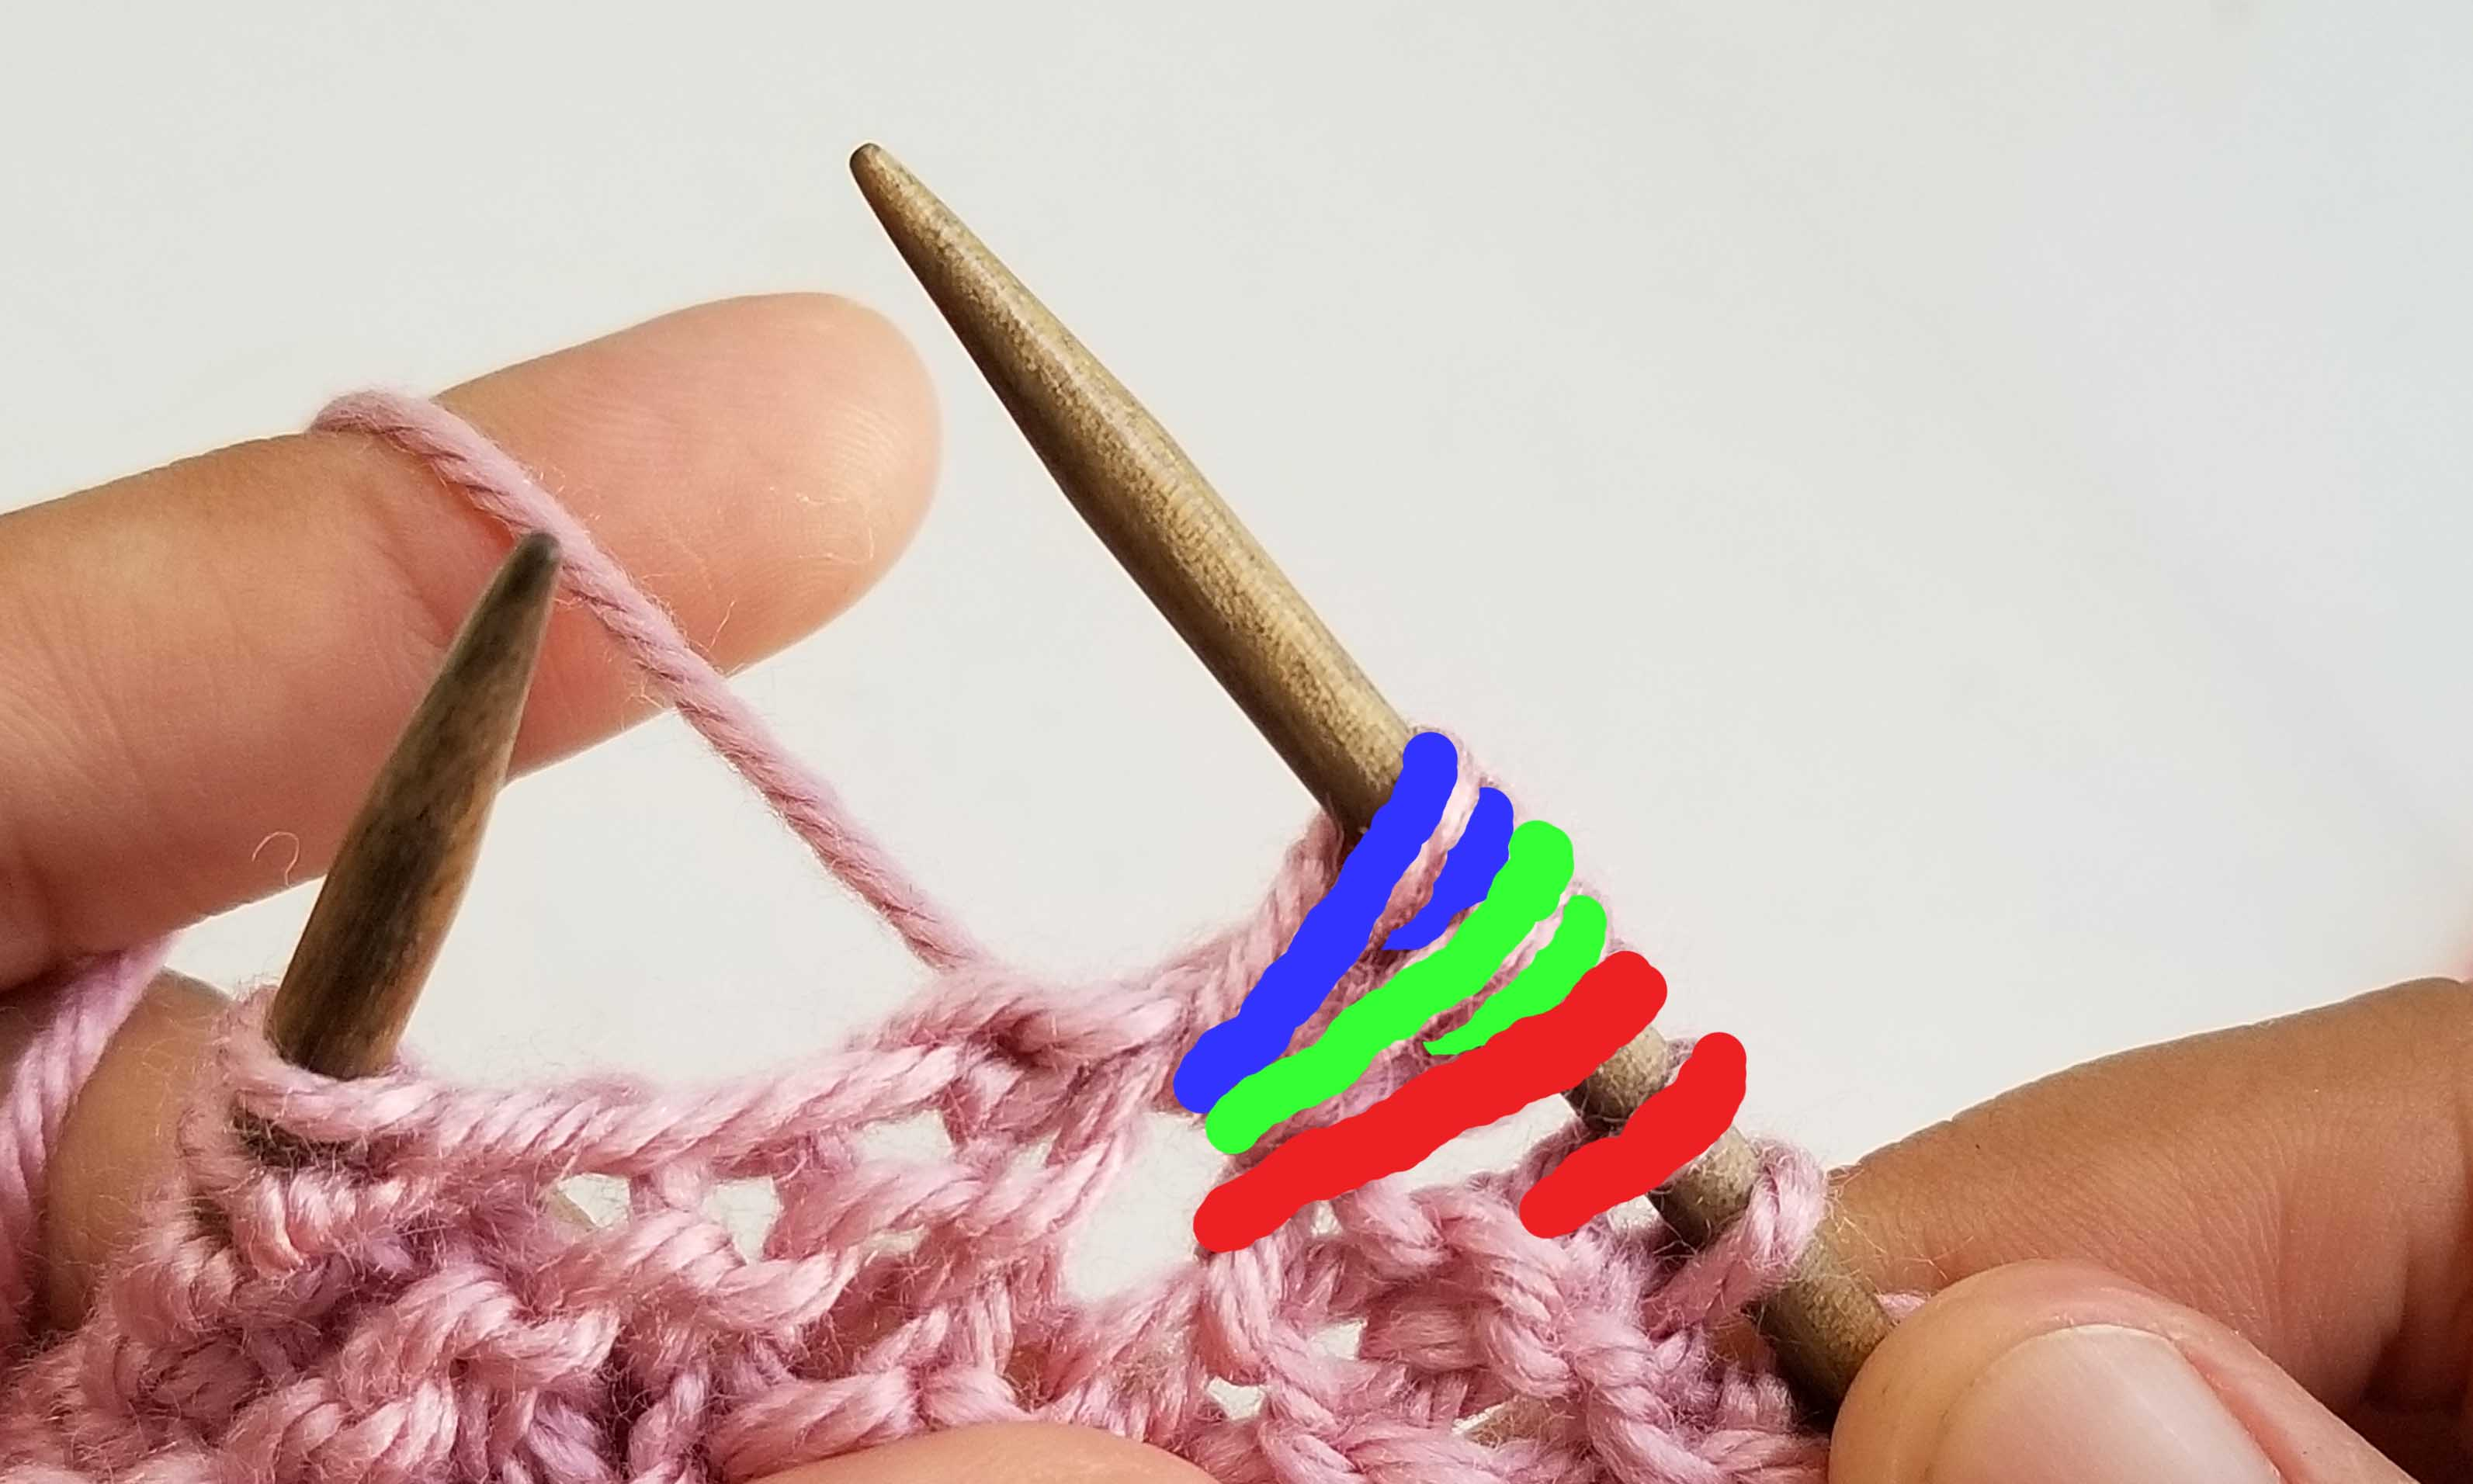
\includegraphics[height=1.5in]{7_loop3.jpg}

\item[7a.] The completed brush stitch (br st): \\
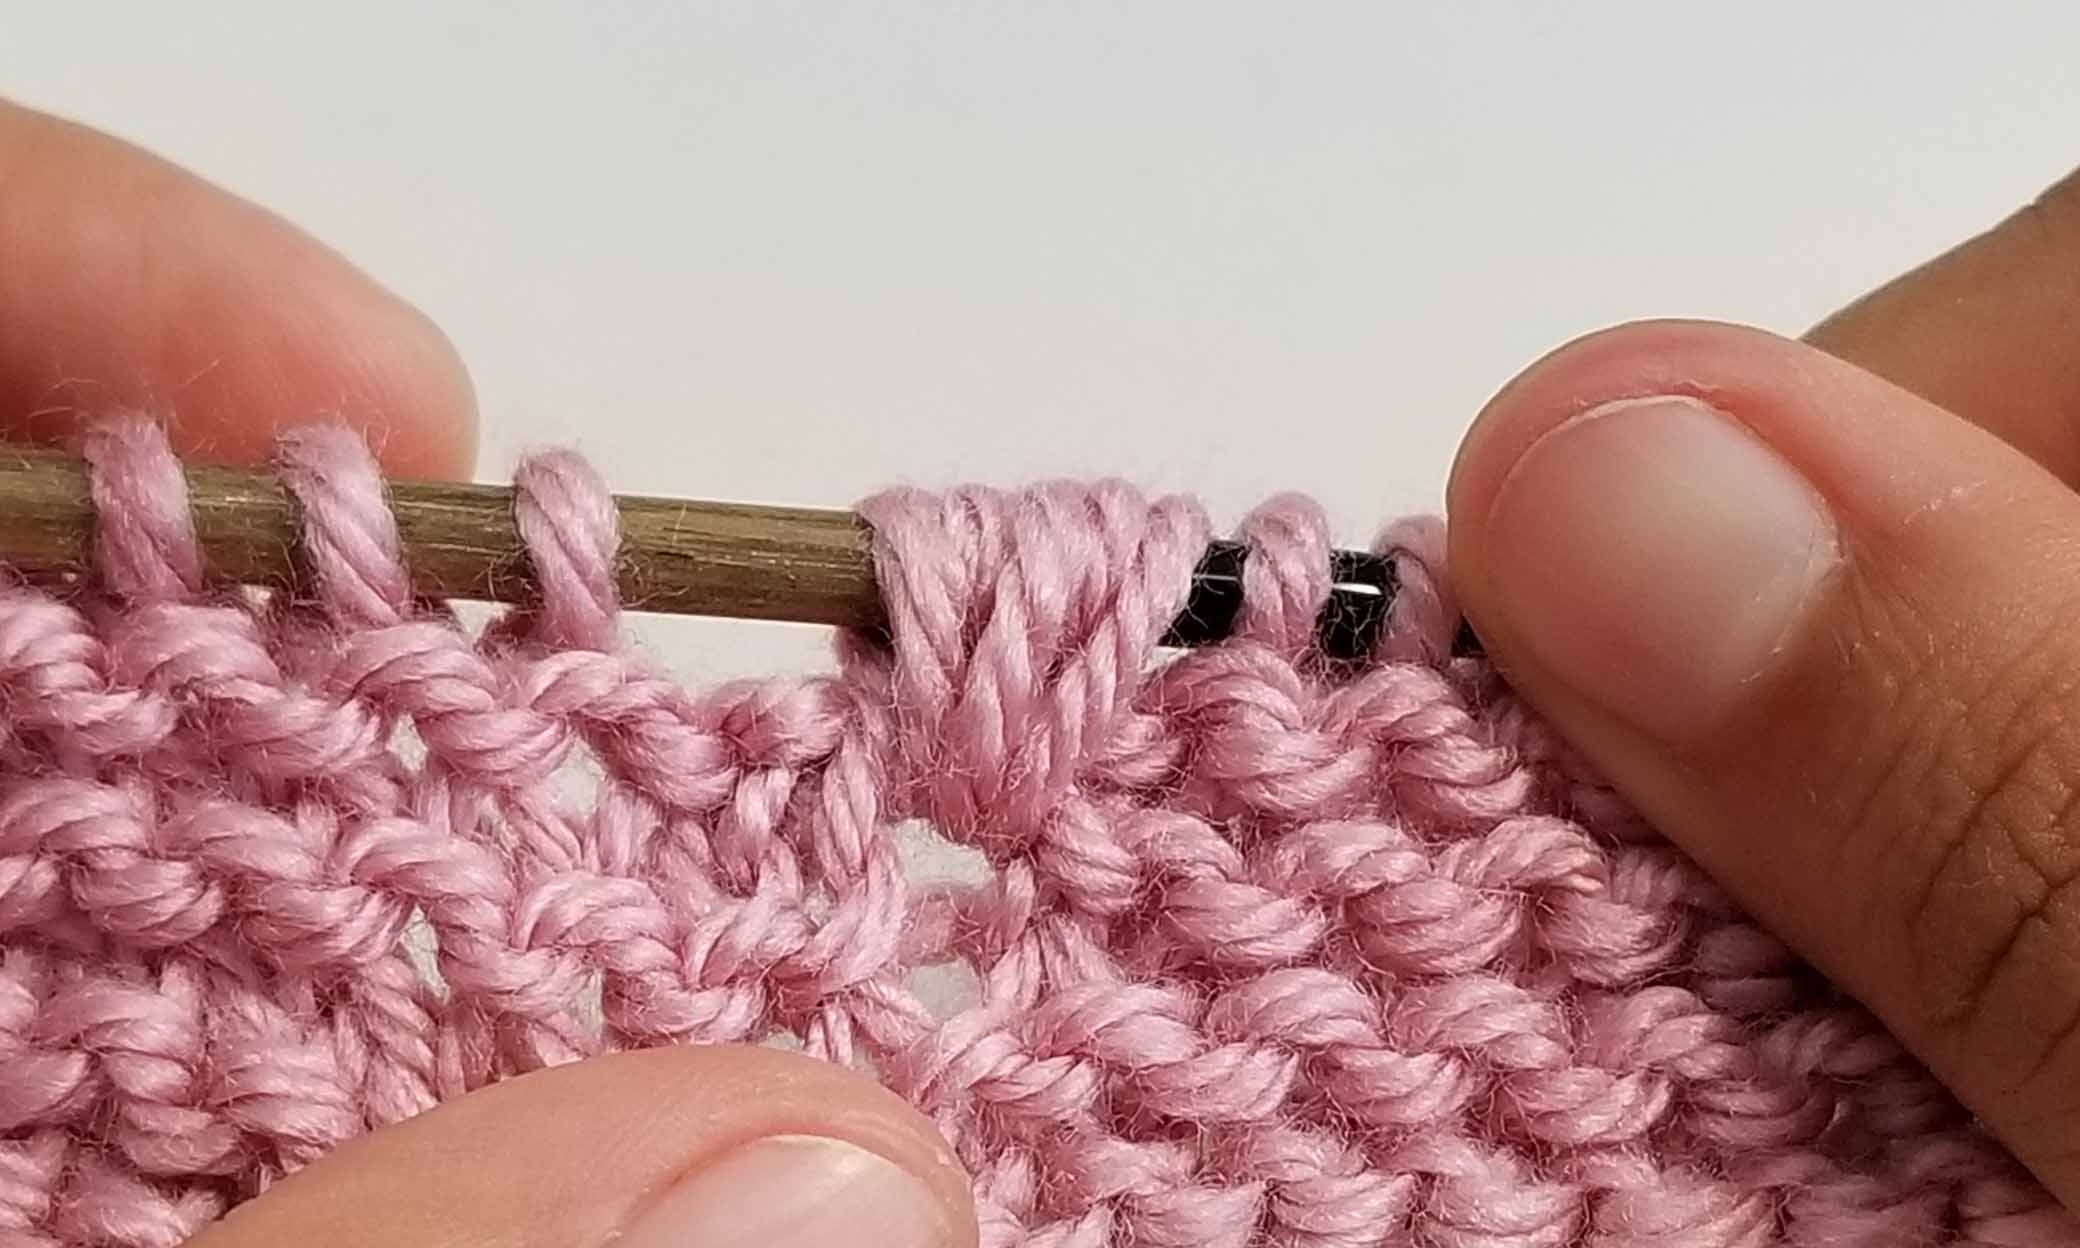
\includegraphics[height=1.5in]{8_finishedRS.jpg}

\item On the following WS row, you will purl together each loop and the stitch after it. \mbox{(i.e. p2tog 1 + 1a, 2 + 2a, and 3 + 3a)} \\
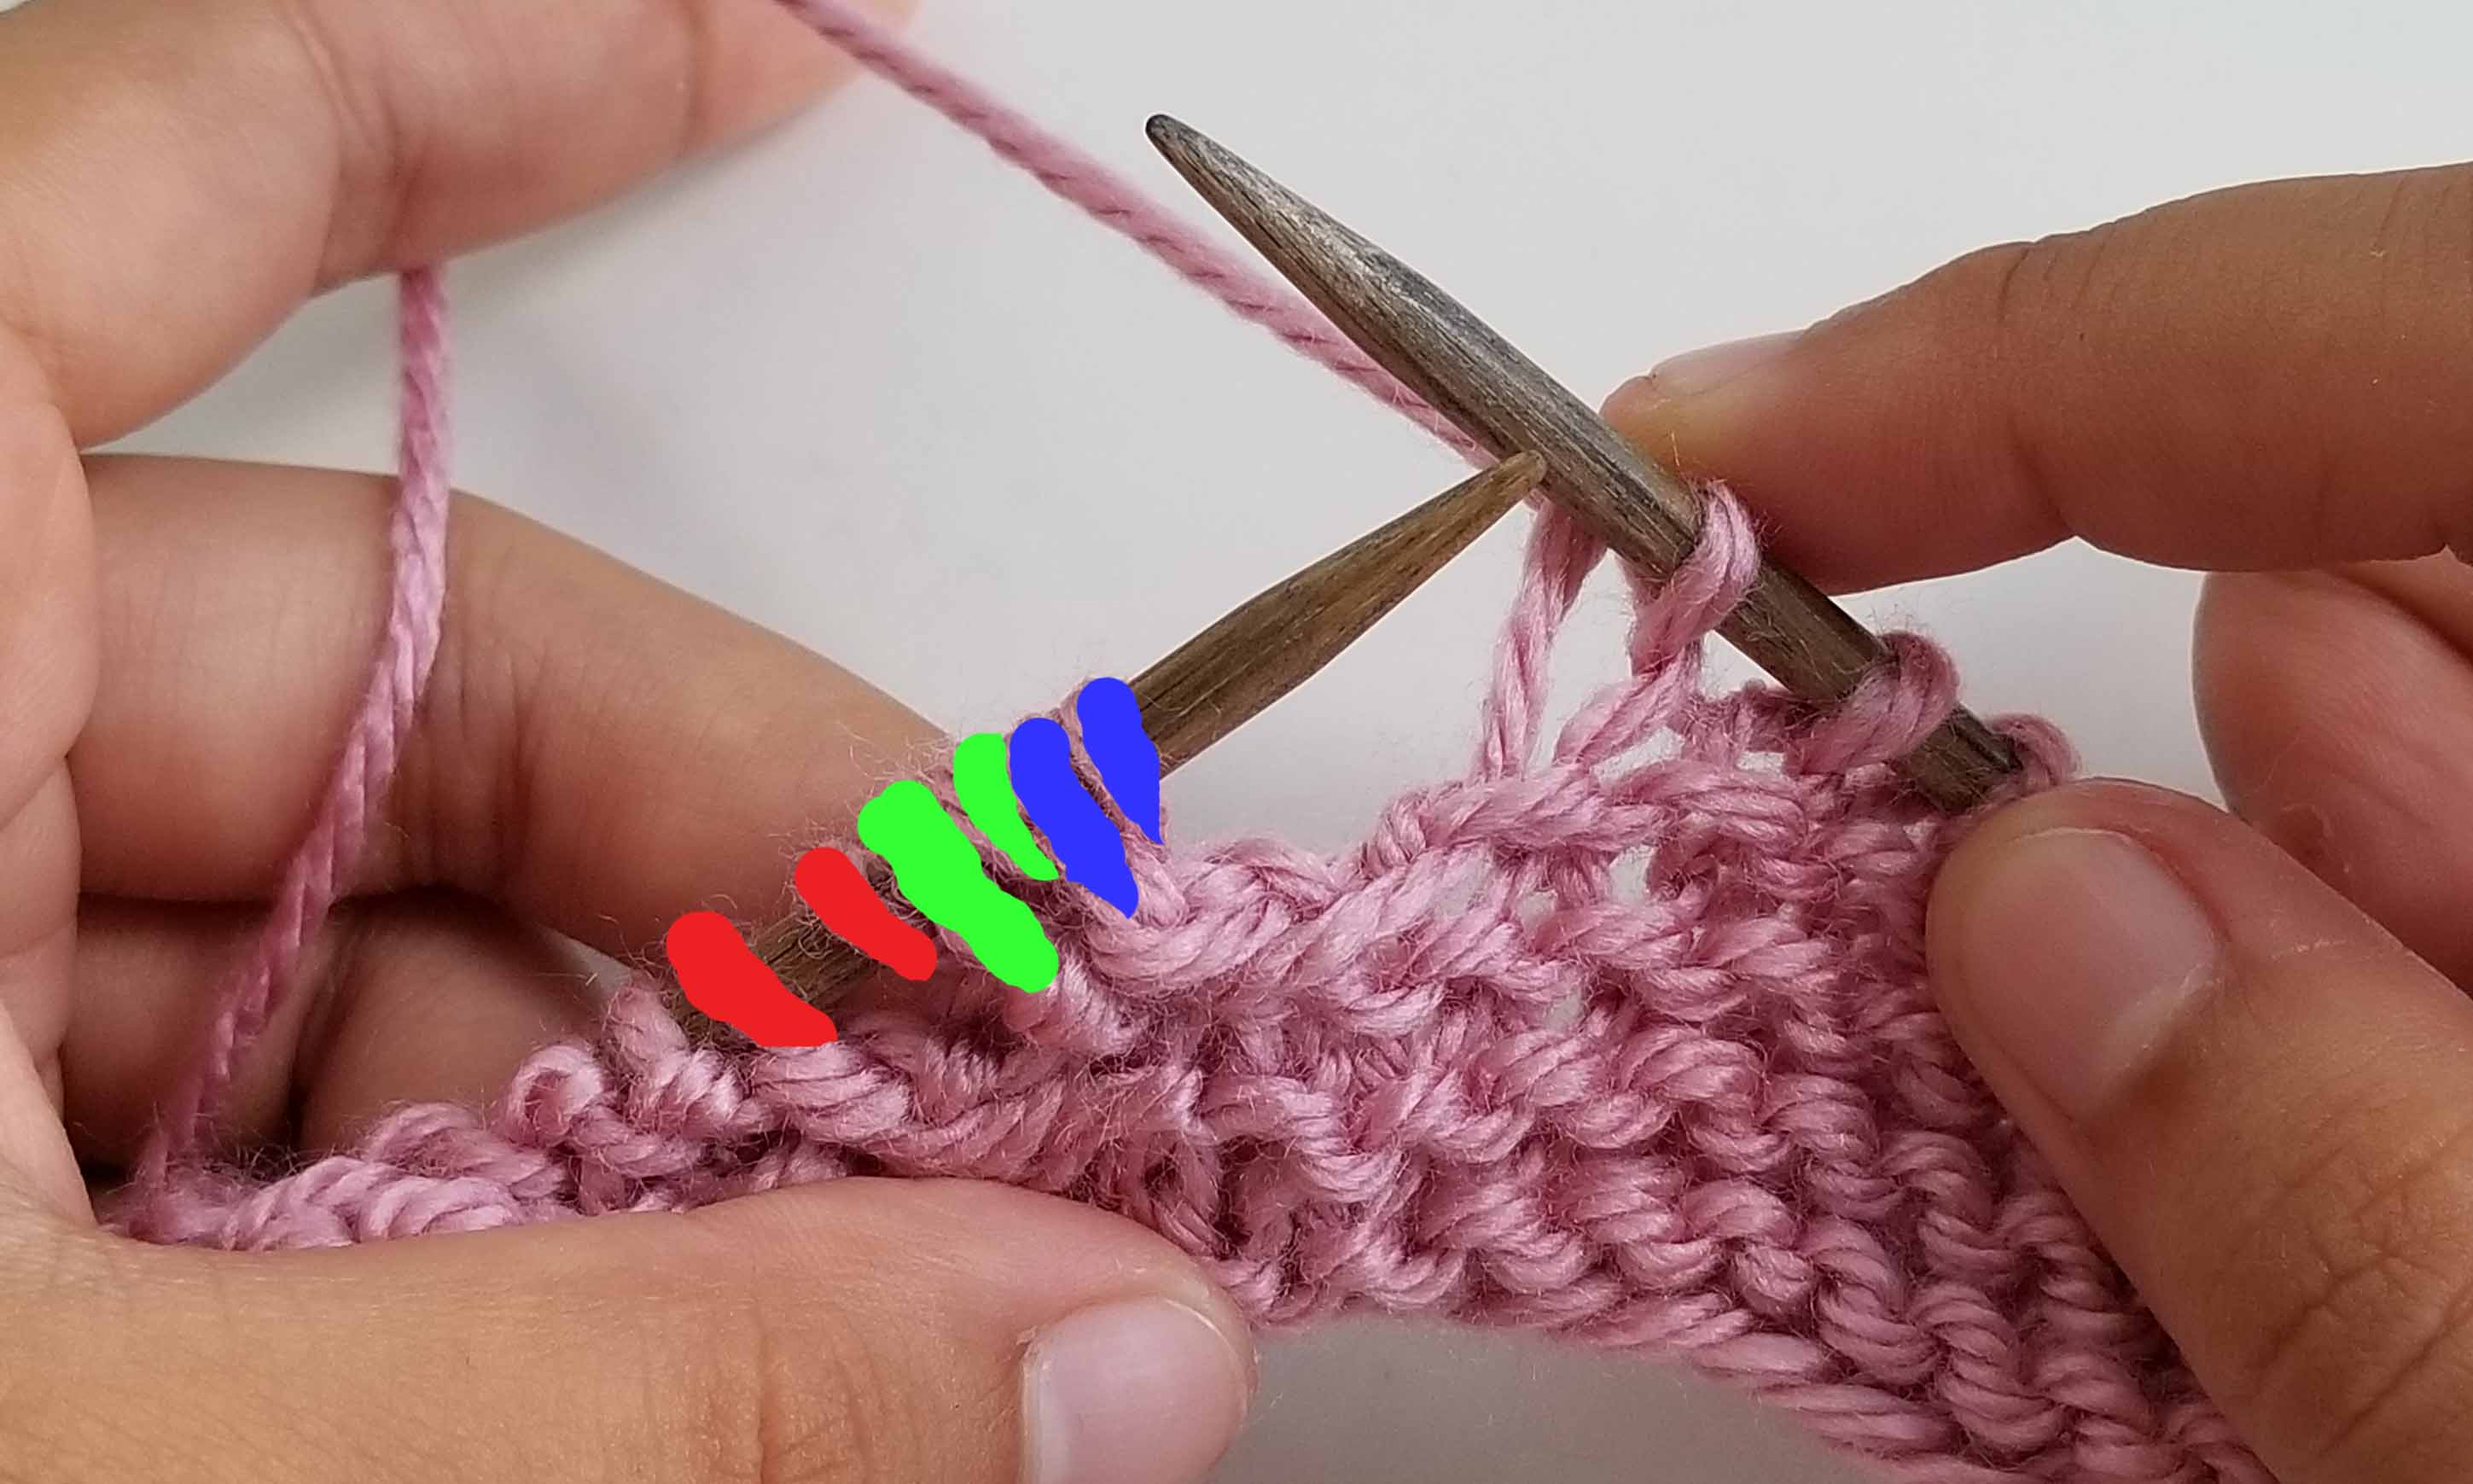
\includegraphics[height=1.5in]{9_WS.jpg}

\item[8a.] Brush stitch after WS row is worked:
\\ 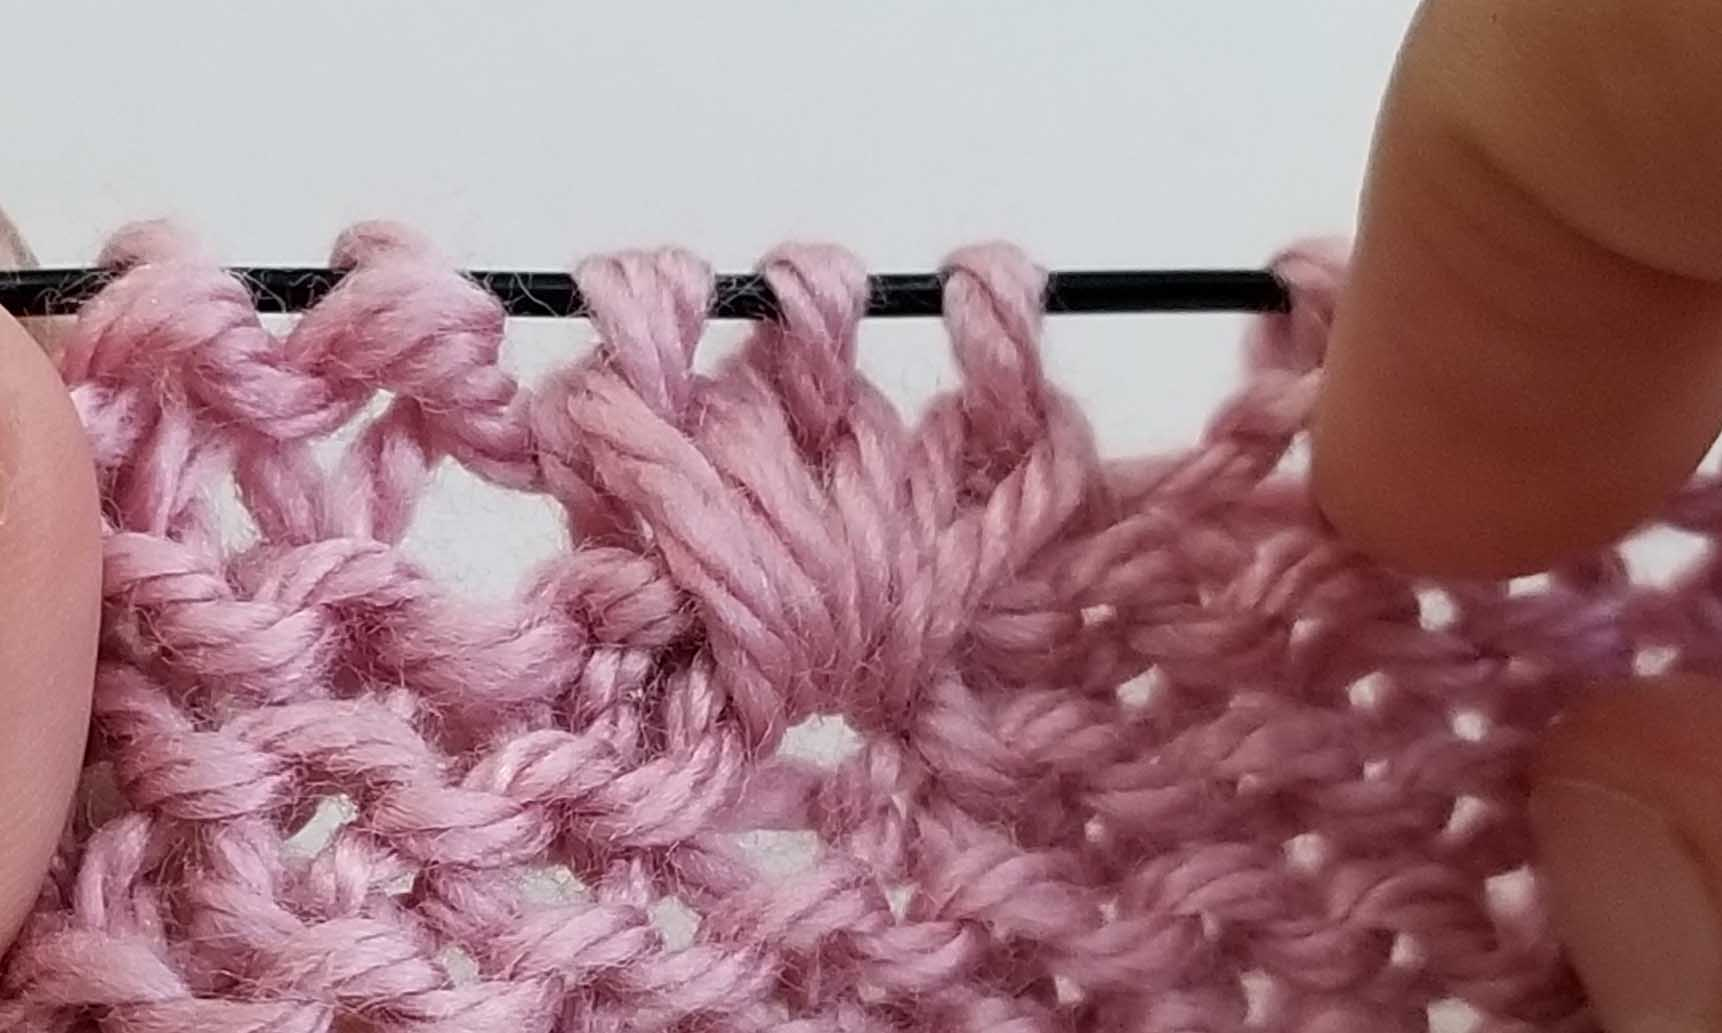
\includegraphics[height=2in]{10_finishedWS.jpg}

\end{enumerate}
\columnbreak

\hspace{1em}\\

\end{multicols}

\end{document}